\chapter{HIỆN THỰC VÀ THỰC NGHIỆM HỆ THỐNG}
\label{ch:chuong4}

\section{Môi trường cài đặt và Công cụ phát triển}
\label{sec:moi_truong_cai_dat}

Toàn bộ hệ thống SmartDorm được xây dựng và triển khai dựa trên các công cụ và phần mềm chuẩn hóa:
\begin{itemize}
    \item \textbf{Môi trường phần cứng và nhúng:} Arduino IDE 2.3.2 kết hợp trình biên dịch ESP32 Core v3.0, Wokwi Simulation Platform, các thư viện ngoại vi chuẩn gồm \texttt{WiFi.h}, \texttt{PubSubClient} (v2.8), \texttt{DHT sensor library} (v1.4.6), và \texttt{MFRC522} (v1.4.11).
    \item \textbf{Môi trường Backend:} Node.js v20 LTS, NestJS CLI v10, TypeScript v5.3, Prisma ORM v5.22, Eclipse Mosquitto MQTT Broker v2.0, Socket.io v4.8.
    \item \textbf{Môi trường Trí tuệ nhân tạo:} Python 3.11, FastAPI v0.110, Uvicorn, Scikit-learn v1.4, XGBoost v2.0, Joblib, Pandas, NumPy, Matplotlib, Seaborn.
    \item \textbf{Môi trường Cơ sở dữ liệu:} PostgreSQL 16 tích hợp extension TimescaleDB (chế độ Production) và SQLite 3 với Prisma Client (chế độ Local Development \& Testing).
    \item \textbf{Môi trường Frontend:} Next.js 16 (App Router), React 19, Tailwind CSS v4, Lucide React Icons, Recharts v3.10, Axios, Zustand.
    \item \textbf{Môi trường kiểm thử tự động:} Jest, Supertest, Playwright Test Automation Engine, Postman, Apache JMeter.
\end{itemize}

\section{Hiện thực phần cứng và Thiết bị nhúng}
\label{sec:hien_thuc_phan_cung}

\subsection{Lập trình Firmware vi điều khiển ESP32}
Firmware trên ESP32 được tổ chức theo kiến trúc máy trạng thái hữu hạn (FSM) kết hợp cơ chế ngắt phần cứng và định thời không khóa (Non-blocking Timer), đảm bảo độ trễ thấp và khả năng hoạt động liên tục:
\begin{enumerate}
    \item \textbf{Quản lý kết nối mạng và MQTT:} Thiết lập cơ chế tự động kết nối lại (Auto-reconnect) với thuật toán hàm mũ ngẫu nhiên (Exponential Backoff) nếu tín hiệu sóng Wi-Fi hoặc Broker bị gián đoạn, ngăn chặn tình trạng nghẽn vi điều khiển.
    \item \textbf{Thu thập dữ liệu cảm biến định kỳ:} Sử dụng bộ đếm thời gian \texttt{millis()} để quét tín hiệu DHT22 và MQ-2 mỗi 5 giây, sau đó đóng gói thành định dạng chuẩn JSON và phát đi qua chủ đề MQTT \texttt{dormitory/+/+/+/sensor/data}.
    \item \textbf{Quét và xử lý thẻ từ RFID:} Vòng lặp liên tục thăm dò thanh ghi module RC522; khi phát hiện có thẻ trong từ trường, đọc mã UID 4-byte, chuyển đổi sang chuỗi Hex chuẩn (ví dụ \texttt{CARD\_A1B2C3D4}) và xuất bản lên chủ đề MQTT để Backend kiểm tra quyền ra vào phòng.
    \item \textbf{Nhận lệnh điều khiển từ xa:} Đăng ký lắng nghe chủ đề \texttt{dormitory/+/+/+/command}. Khi nhận lệnh đóng/ngắt relay từ Backend, firmware kích hoạt ngay mức logic tương ứng tại các chân GPIO 25, 14, 12, 13 và phản hồi gói tin xác nhận \texttt{command/ack}.
    \item \textbf{Cơ chế an toàn tại chỗ (Local Fail-Safe):} Trong trường hợp mất kết nối mạng đến máy chủ, nếu cảm biến MQ-2 đo được nồng độ gas $\ge 80\%$, vi điều khiển tự động ngắt toàn bộ relay và hú còi cảnh báo tại chỗ mà không cần chờ lệnh từ Backend.
\end{enumerate}

\subsection{Hình ảnh thực tế mô hình phần cứng}

\begin{figure}[H]
    \centering
    \setlength{\fboxsep}{10pt}
    \setlength{\fboxrule}{1.5pt}
    \fbox{%
        \begin{minipage}{0.88\textwidth}
            \centering
            \vspace{2.5cm}
            \textbf{\Large [CHỖ TRỐNG CHÈN ẢNH MẠCH THIẾT BỊ PHẦN CỨNG THỰC TẾ]}\\[0.4cm]
            \textit{(Khu vực dành riêng cho việc bổ sung hình ảnh chụp thực tế mô hình phần cứng hoàn chỉnh gồm vi điều khiển ESP32 DevKit V1, module Relay 4 kênh cách ly quang, cảm biến vi khí hậu DHT22, cảm biến gas MQ-2, đầu đọc thẻ RFID RC522 và còi báo động sau khi hoàn thiện đóng hộp thiết bị tại phòng KTX)}\\[0.2cm]
            \vspace{2.5cm}
        \end{minipage}%
    }
    \caption{Mô hình lắp ráp mạch điều khiển phần cứng thực tế tại phòng KTX}
    \label{fig:hardware_real_placeholder}
\end{figure}

\begin{figure}[H]
    \centering
    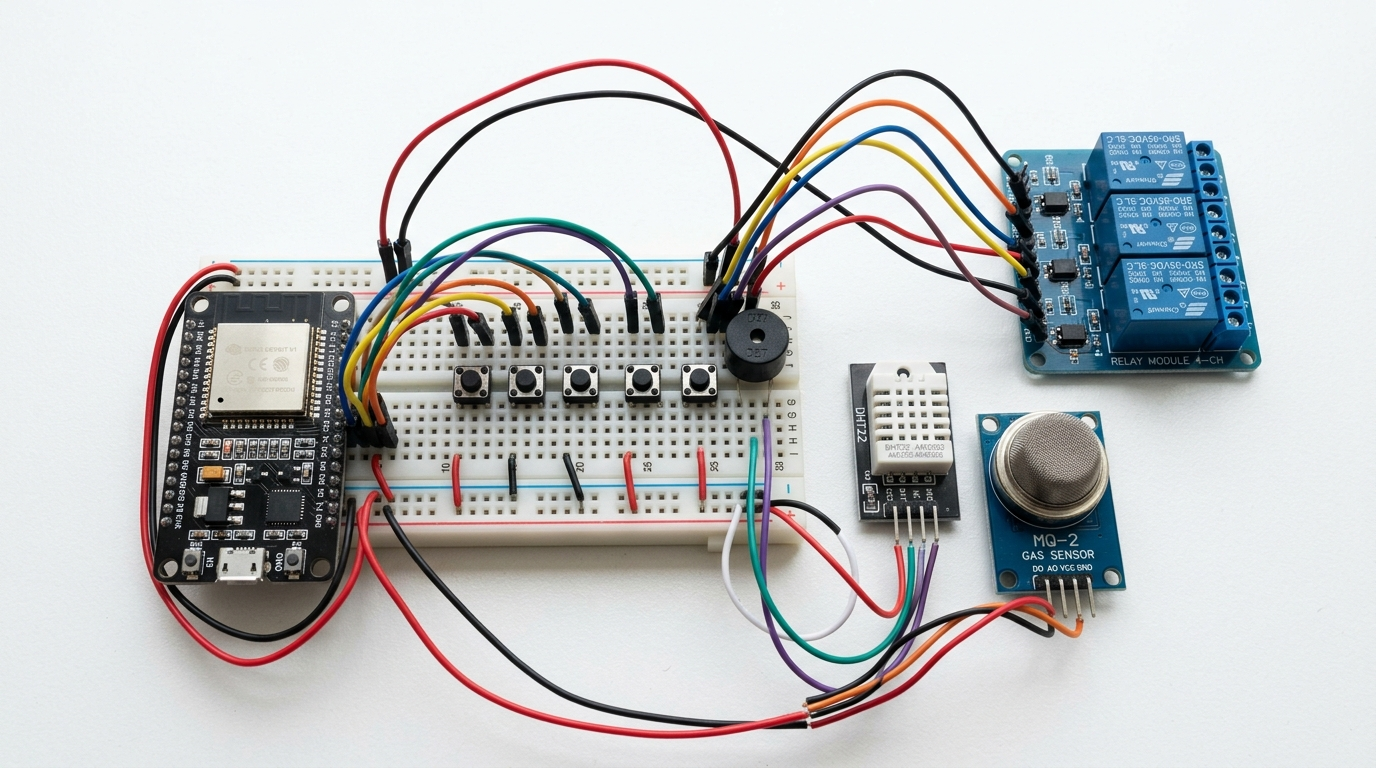
\includegraphics[width=0.75\textwidth]{figures/tong_the_lap_rap.jpg}
    \caption{Mô hình lắp ráp thí nghiệm tổng thể các module cảm biến và cơ cấu chấp hành}
    \label{fig:hardware_assembly_overview}
\end{figure}

\section{Hiện thực hệ thống phần mềm và Giao diện chức năng}
\label{sec:hien_thuc_phan_mem}

Hệ thống SmartDorm được thiết kế với giao diện Dark Mode cao cấp, bố cục trực quan, hỗ trợ đầy đủ các thao tác nghiệp vụ cho cả Quản trị viên và Sinh viên. Dưới đây là hình ảnh thực tế và mô tả chi tiết từng chức năng được chụp trực tiếp từ hệ thống đang vận hành:

\subsection{Giao diện Đăng nhập và Xác thực bảo mật}
Màn hình đăng nhập (Hình~\ref{fig:ss_login}) cung cấp cơ chế xác thực an toàn thông qua Email và Mật khẩu. Hệ thống hỗ trợ đăng nhập cho cả cán bộ quản trị và sinh viên. Khi đăng nhập thành công, máy chủ NestJS cấp phát mã thông báo JWT (JSON Web Token) chứa định danh người dùng và vai trò phân quyền (Role: \texttt{ADMIN}, \texttt{STUDENT}, \texttt{STAFF}), từ đó tự động điều hướng người dùng về đúng phân hệ tương ứng.

\begin{figure}[H]
    \centering
    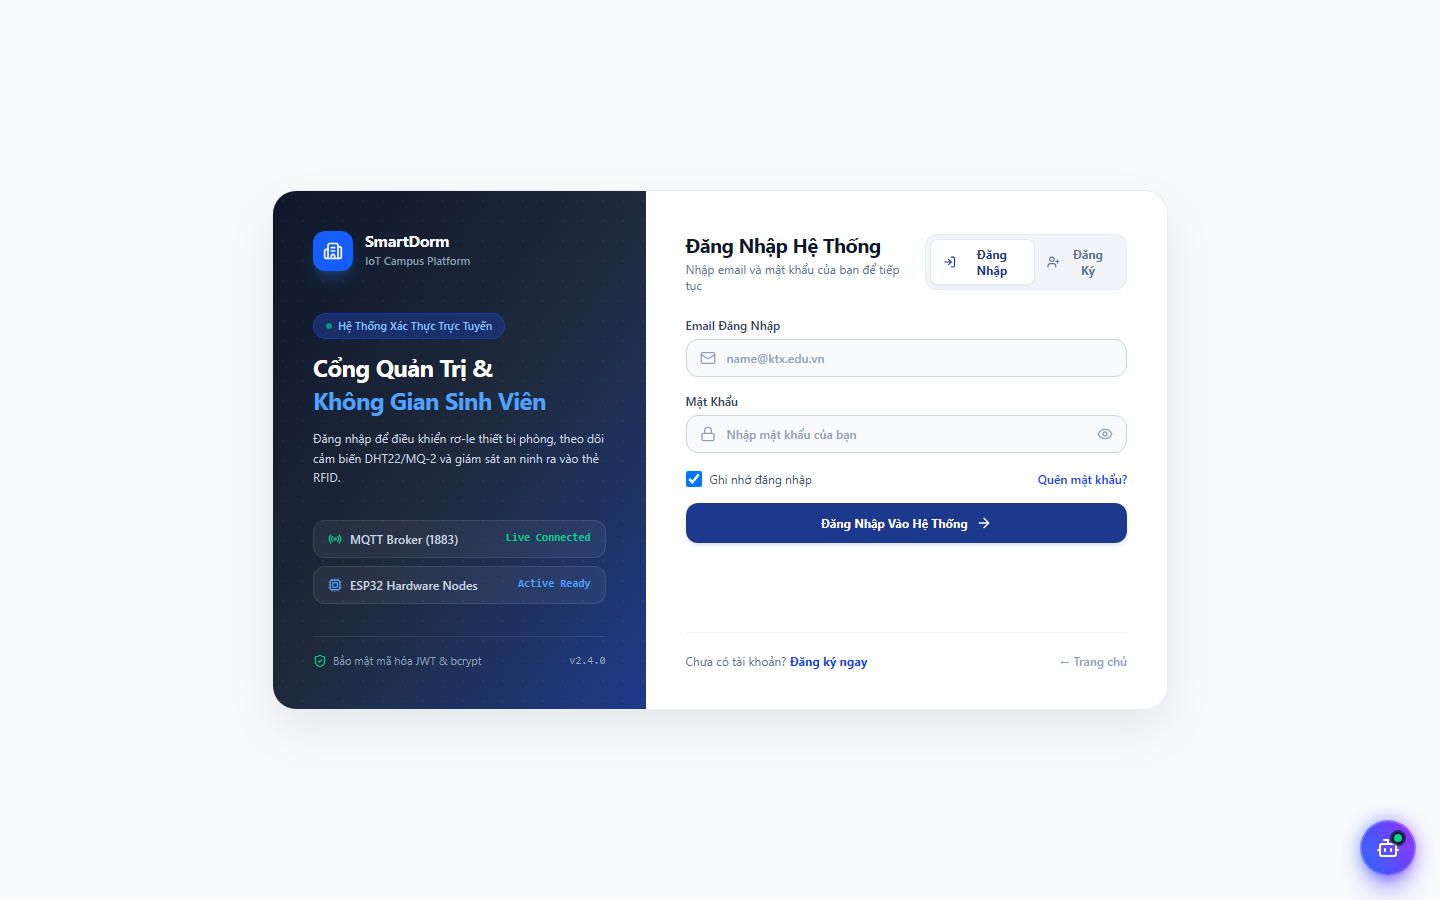
\includegraphics[width=0.88\textwidth]{figures/screenshots/01_login_page.png}
    \caption{Giao diện Đăng nhập hệ thống SmartDorm (Next.js 16)}
    \label{fig:ss_login}
\end{figure}

\subsection{Phân hệ Quản trị viên (Admin Portal)}

\subsubsection{Bảng điều khiển tổng quan KPI (Dashboard Overview)}
Giao diện Dashboard tổng quan (Hình~\ref{fig:ss_admin_dashboard}) hiển thị các thẻ số liệu thống kê thời gian thực quan trọng: Tổng số phòng đang quản lý (18 phòng), Số lượng sinh viên nội trú (18 sinh viên), Tổng số thiết bị IoT đang trực tuyến (72 thiết bị), Mức công suất phụ tải tức thời và Số lượng cảnh báo an toàn đang kích hoạt. Biểu đồ vi khí hậu trực quan hóa sự biến thiên của nhiệt độ và độ ẩm phòng theo thời gian thông qua thư viện Recharts.

\begin{figure}[H]
    \centering
    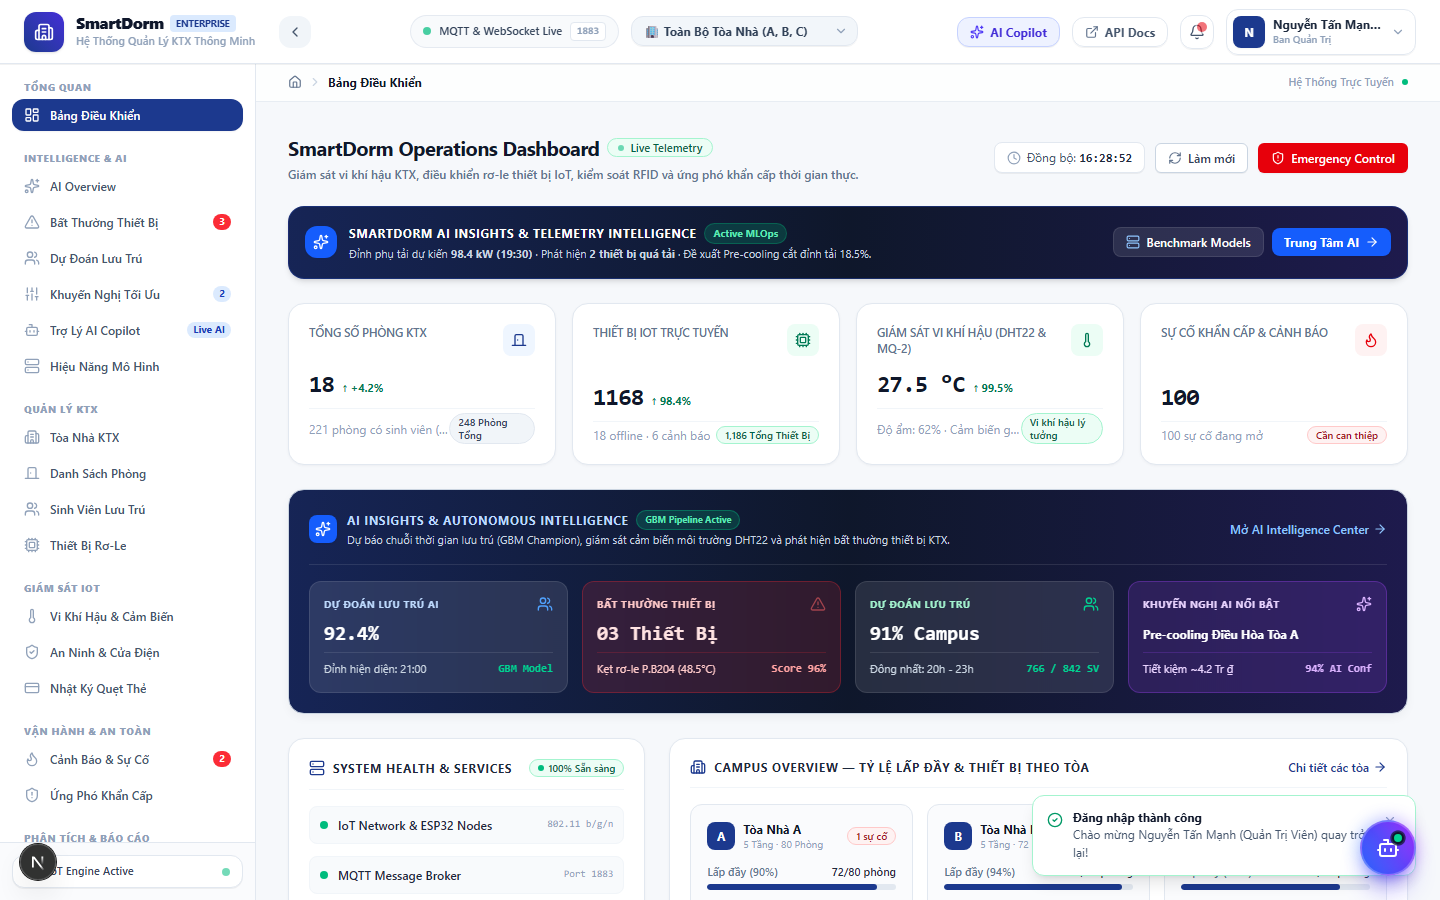
\includegraphics[width=0.88\textwidth]{figures/screenshots/02_admin_dashboard.png}
    \caption{Bảng điều khiển tổng quan KPI dành cho Quản trị viên}
    \label{fig:ss_admin_dashboard}
\end{figure}

\subsubsection{Quản lý Tòa nhà, Phòng ở và Phân bổ sinh viên}
Màn hình Quản lý Phòng (Hình~\ref{fig:ss_admin_rooms}) cho phép quản trị viên xem danh mục các phòng theo từng tòa nhà (Tòa A, Tòa B, Tòa C). Với mỗi phòng, hệ thống hiển thị chi tiết sức chứa, số giường trống, danh sách bạn cùng phòng và trạng thái thiết bị điện. Khi một sinh viên được phân bổ vào phòng, hệ thống tự động kích hoạt thuật toán sinh mã thẻ từ RFID tương ứng.

\begin{figure}[H]
    \centering
    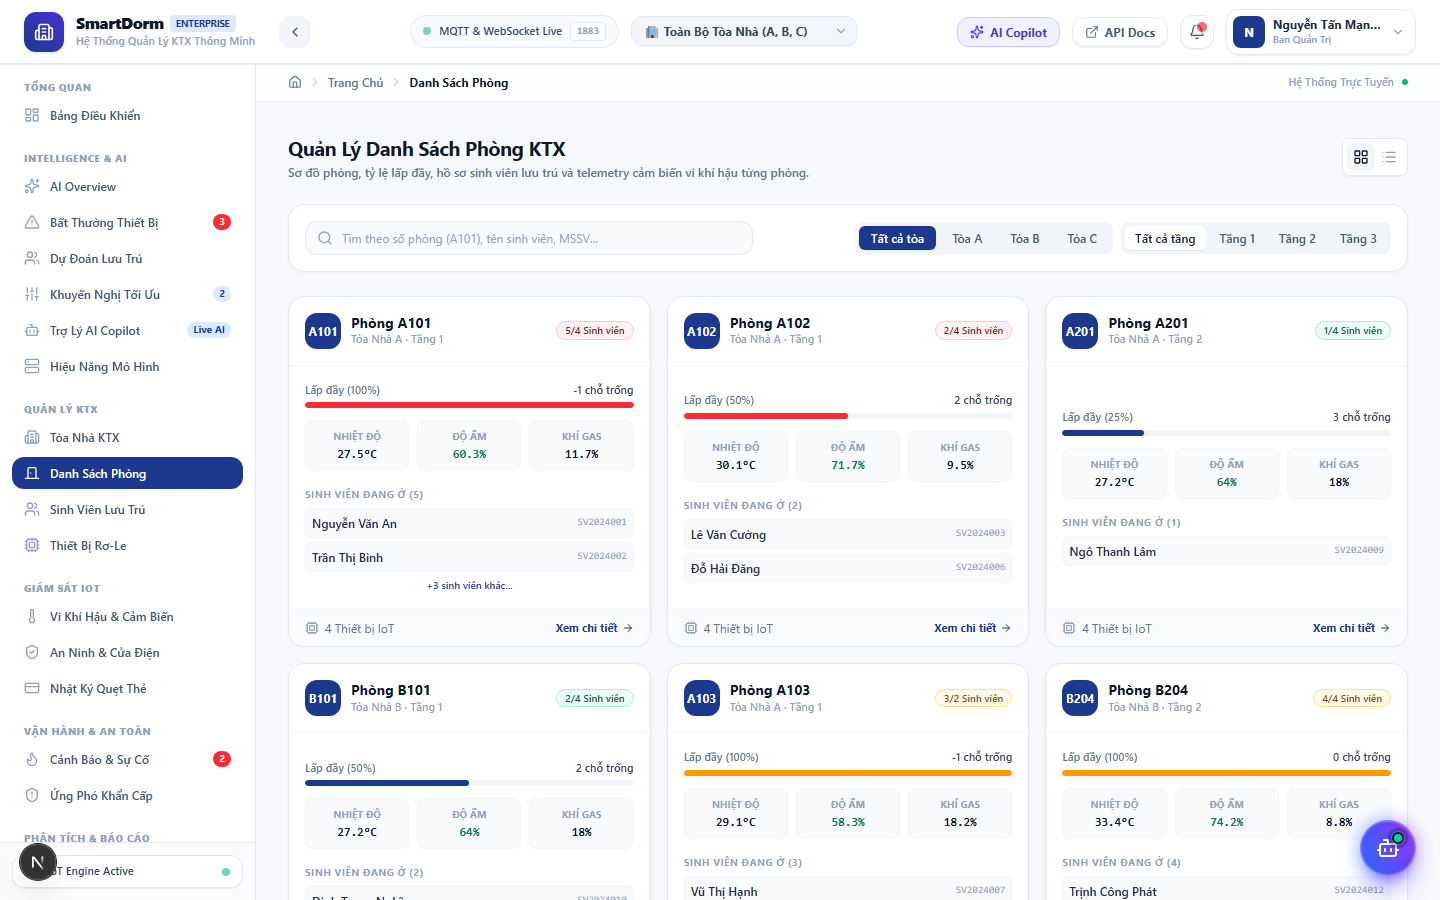
\includegraphics[width=0.88\textwidth]{figures/screenshots/03_admin_rooms.png}
    \caption{Giao diện Quản lý danh mục phòng ở và phân bổ cư dân}
    \label{fig:ss_admin_rooms}
\end{figure}

\subsubsection{Điều khiển thiết bị thời gian thực và Khả năng Hoàn tác lệnh (Undo Command)}
Giao diện Điều khiển Thiết bị (Hình~\ref{fig:ss_admin_devices}) cung cấp các công tắc chuyển mạch số (Toggle Switch) cho phép bật/tắt tức thời đèn chiếu sáng, quạt thông gió, máy điều hòa và chốt khóa cửa điện từ. Hệ thống triển khai mẫu thiết kế Command Pattern: mỗi lệnh gửi qua MQTT được lưu vào bảng lịch sử \texttt{CommandHistory}, hiển thị nút ``Hoàn tác lệnh'' (Undo Last Command) giúp quản trị viên dễ dàng khôi phục trạng thái ban đầu của thiết bị nếu bấm nhầm.

\begin{figure}[H]
    \centering
    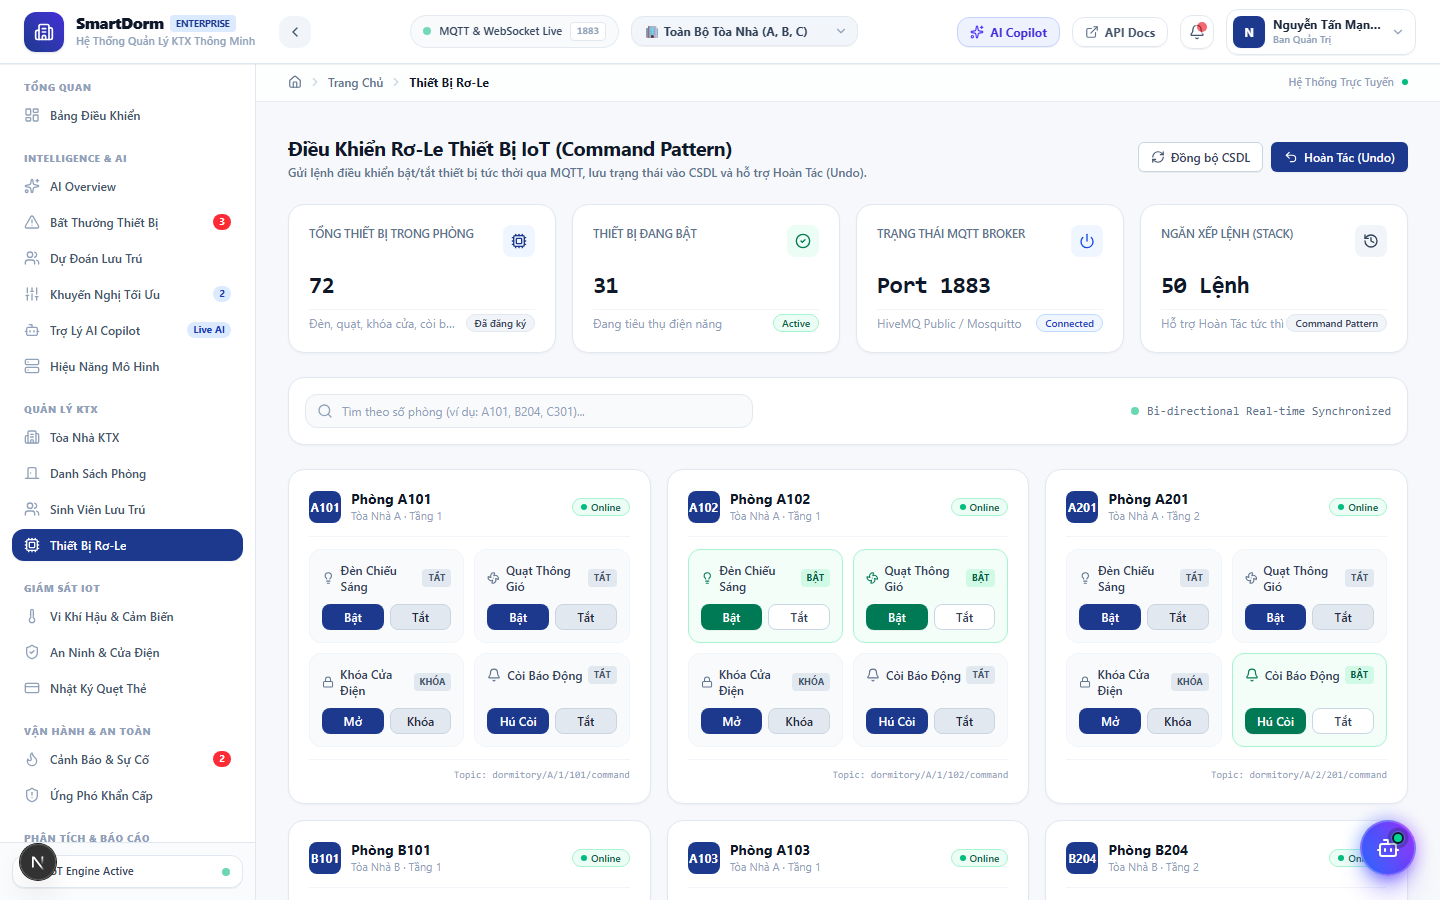
\includegraphics[width=0.88\textwidth]{figures/screenshots/04_admin_devices.png}
    \caption{Giao diện Điều khiển thiết bị và Lịch sử lệnh có hỗ trợ Hoàn tác (Undo)}
    \label{fig:ss_admin_devices}
\end{figure}

\subsubsection{Nhật ký Quẹt thẻ RFID và Giám sát An ninh}
Màn hình Nhật ký Ra vào (Hình~\ref{fig:ss_admin_access}) ghi nhận chi tiết toàn bộ các sự kiện quẹt thẻ RFID tại các phòng: thời gian chính xác, mã thẻ, mã sinh viên, tên sinh viên và trạng thái hợp lệ. Các lượt quẹt thẻ thành công được đánh dấu nhãn xanh lá (Granted - Entry/Exit), trong khi các lượt quẹt thẻ không hợp lệ hoặc trái phép được đánh dấu nhãn đỏ (Denied), hỗ trợ truy vết an ninh kịp thời.

\begin{figure}[H]
    \centering
    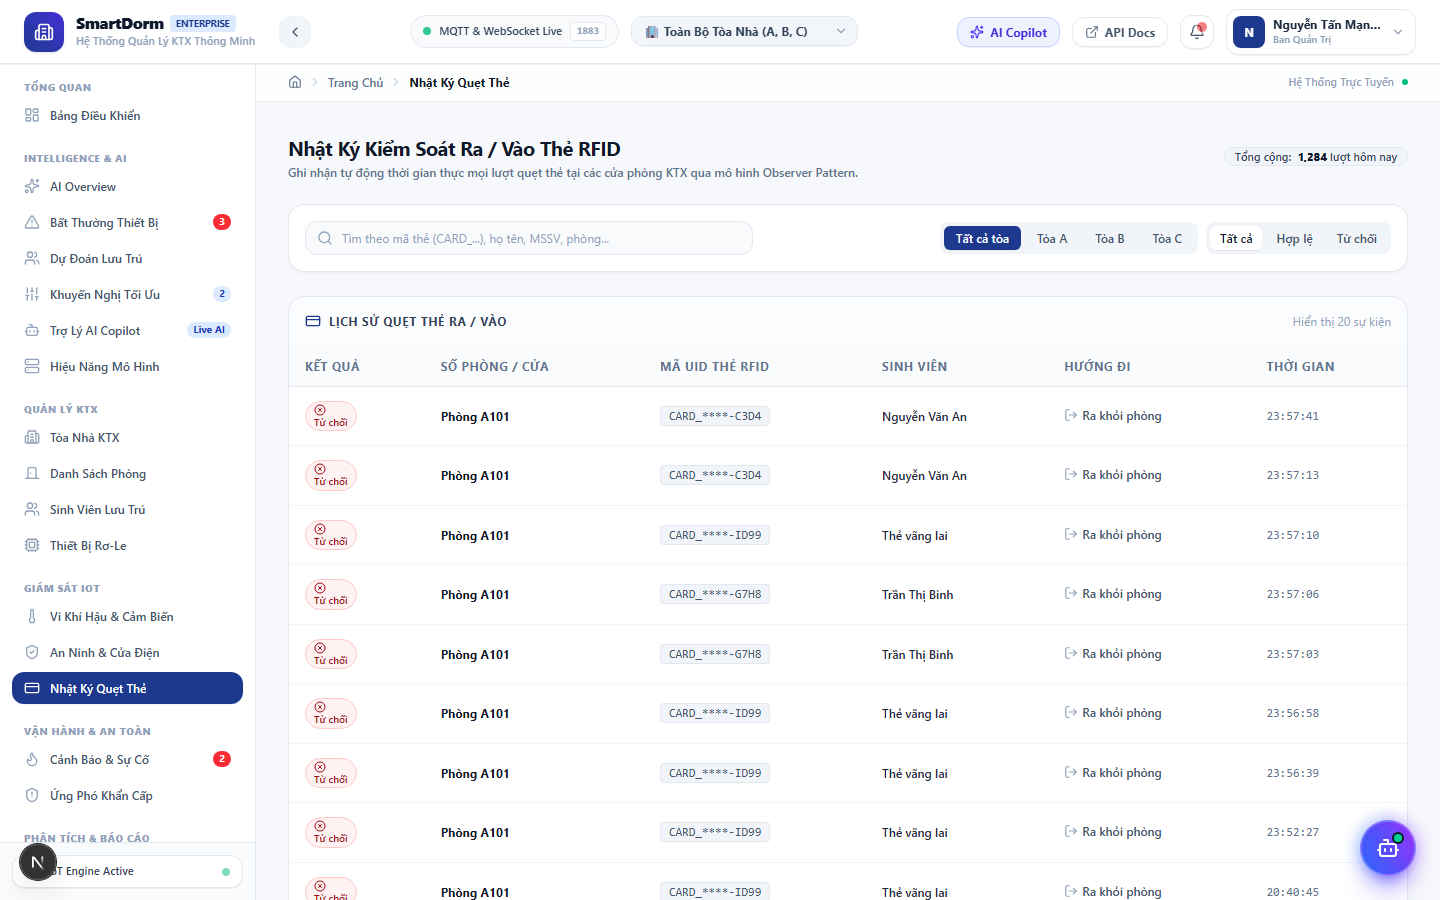
\includegraphics[width=0.88\textwidth]{figures/screenshots/05_admin_access_logs.png}
    \caption{Giao diện Nhật ký quẹt thẻ RFID kiểm soát an ninh ra vào}
    \label{fig:ss_admin_access}
\end{figure}

\subsubsection{Trung tâm phản ứng sự cố khẩn cấp PCCC}
Màn hình Cảnh báo Khẩn cấp (Hình~\ref{fig:ss_admin_emergency}) hiển thị danh sách các sự cố cháy nổ, rò rỉ khí gas hoặc quá nhiệt độ môi trường. Khi cảm biến MQ-2 ghi nhận nồng độ gas $\ge 80\%$, hệ thống tự động kích hoạt cơ chế an toàn: ngắt toàn bộ relay điện phòng để triệt tiêu nguồn phát tia lửa, mở khóa cửa điện từ để thoát hiểm, và hiển thị banner cảnh báo đỏ khẩn cấp trên toàn màn hình. Quản trị viên có thể bấm nút ``Đánh dấu đã xử lý'' (Resolve) sau khi đội kỹ thuật hoàn tất khắc phục tại hiện trường.

\begin{figure}[H]
    \centering
    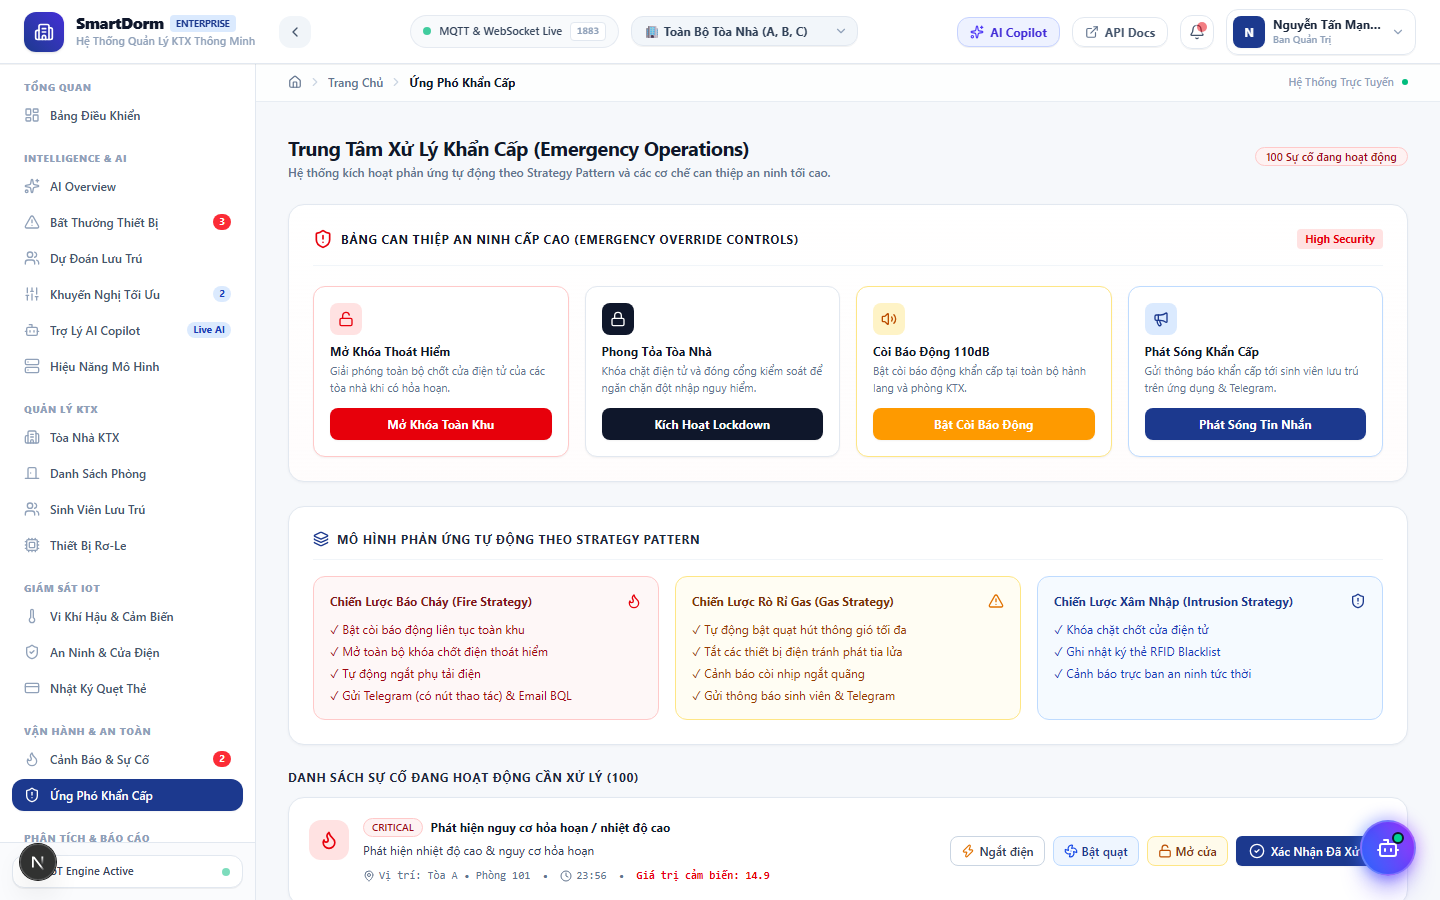
\includegraphics[width=0.88\textwidth]{figures/screenshots/06_admin_emergency.png}
    \caption{Trung tâm giám sát và xử lý cảnh báo sự cố khẩn cấp PCCC}
    \label{fig:ss_admin_emergency}
\end{figure}

\subsubsection{Báo cáo phân tích Business Intelligence (BI Analytics)}
Trang Phân tích BI (Hình~\ref{fig:ss_admin_analytics}) tổng hợp các chỉ số vận hành chuyên sâu của ký túc xá qua các biểu đồ phân tích đa chiều: phân phối mức tiêu thụ điện năng theo khung giờ cao điểm/thấp điểm, tỷ lệ vi phạm an ninh ra vào, thống kê sự cố thiết bị và chức năng xuất dữ liệu báo cáo sang định dạng Excel/CSV.

\begin{figure}[H]
    \centering
    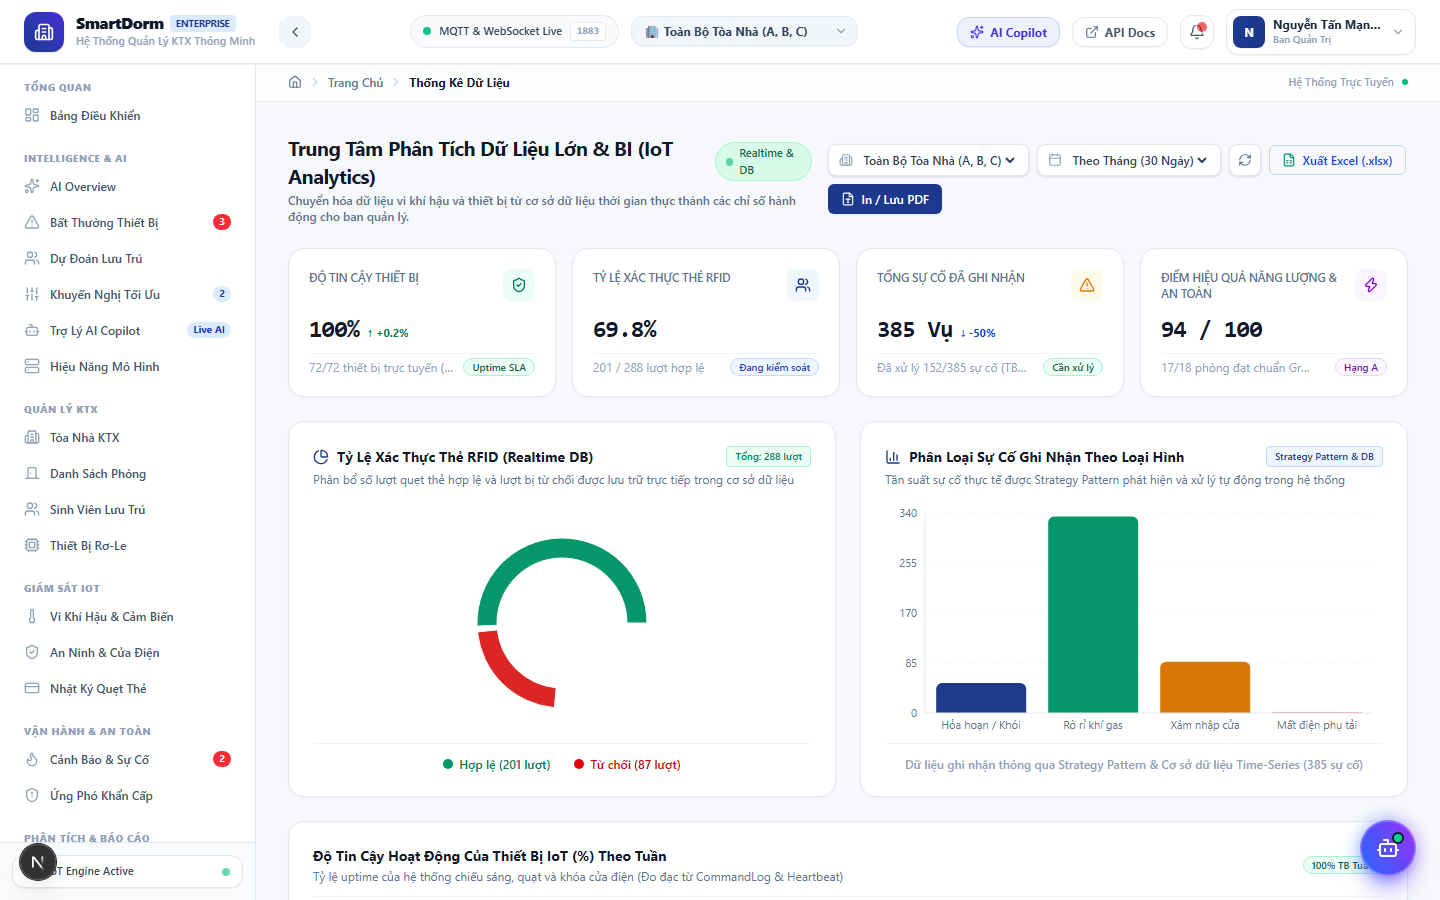
\includegraphics[width=0.88\textwidth]{figures/screenshots/07_admin_analytics.png}
    \caption{Báo cáo phân tích kinh doanh (BI) và thống kê vận hành KTX}
    \label{fig:ss_admin_analytics}
\end{figure}

\subsubsection{Giám sát phụ tải năng lượng điện}
Giao diện Giám sát Năng lượng (Hình~\ref{fig:ss_admin_energy}) cung cấp biểu đồ Recharts đường xu hướng tiêu thụ điện năng của toàn bộ các tòa nhà và từng phòng theo thời gian thực (được tính toán chính xác bằng mô hình Digital Proxy). Hệ thống tự động tính toán hóa đơn tiền điện dự kiến theo biểu giá điện sinh hoạt bậc thang EVN.

\begin{figure}[H]
    \centering
    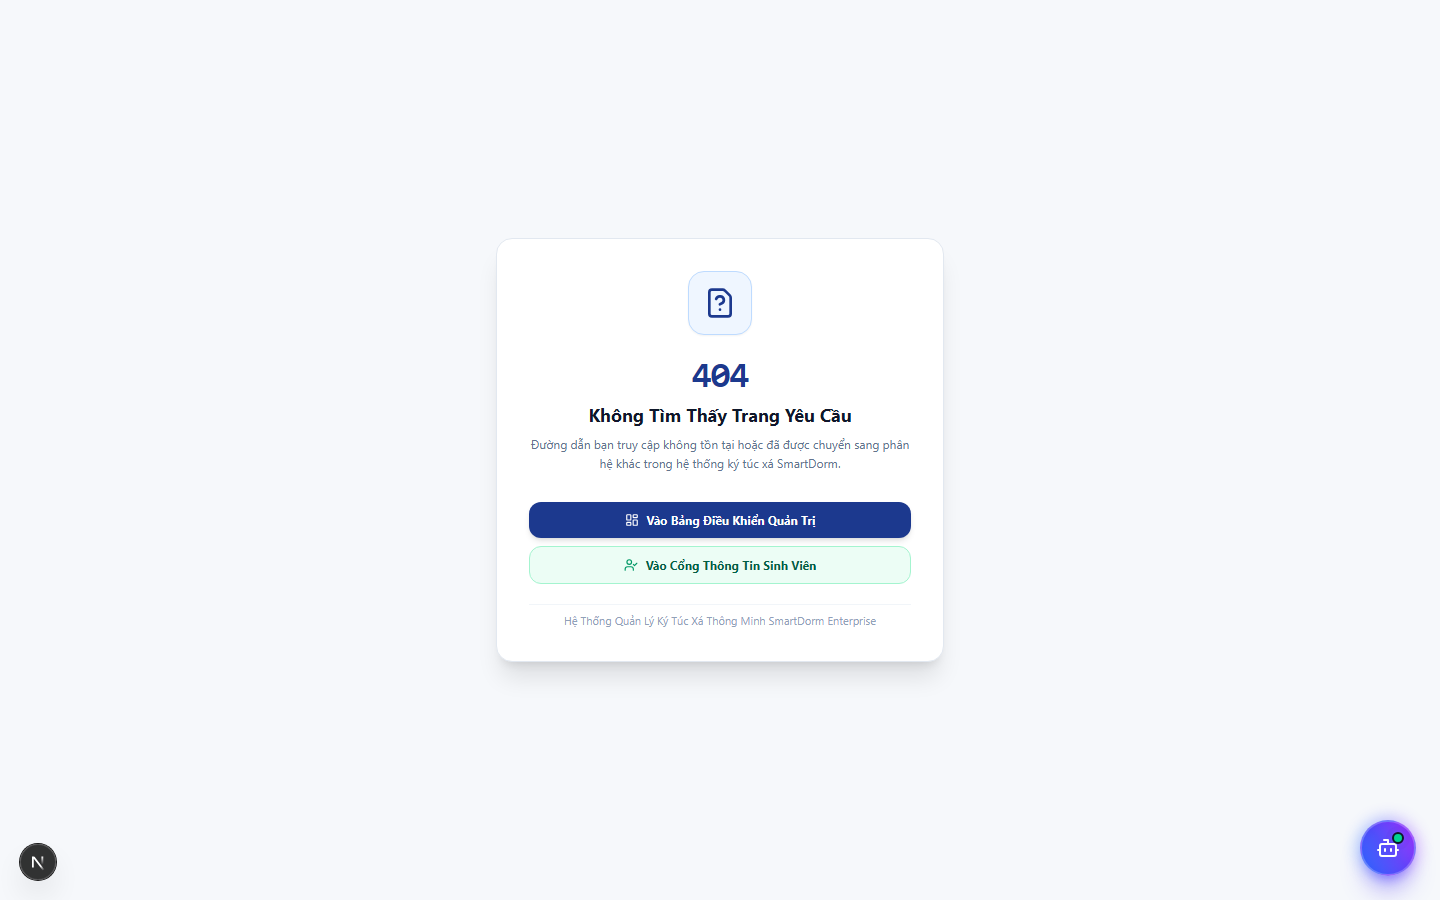
\includegraphics[width=0.88\textwidth]{figures/screenshots/08_admin_energy.png}
    \caption{Giao diện Giám sát phụ tải điện năng và biểu giá EVN}
    \label{fig:ss_admin_energy}
\end{figure}

\subsubsection{Trung tâm Quản trị Mô hình Trí tuệ nhân tạo (AI Models Center)}
Giao diện Quản trị AI (Hình~\ref{fig:ss_admin_ai_models}) cho phép cán bộ kỹ thuật theo dõi tình trạng sức khỏe của các mô hình học máy: mô hình Champion GBM (Dự báo phụ tải điện năng 24h), mô hình Isolation Forest (Phát hiện bất thường thiết bị), và mô hình Occupancy Proxy Classifier. Màn hình hiển thị đầy đủ các chỉ số định lượng MAE, RMSE, F1-Score, độ trễ suy luận (Latency) và biểu đồ phát hiện trôi dạt dữ liệu (Data Drift / Model Drift) kèm nút kích hoạt huấn luyện lại (Retrain Model).

\begin{figure}[H]
    \centering
    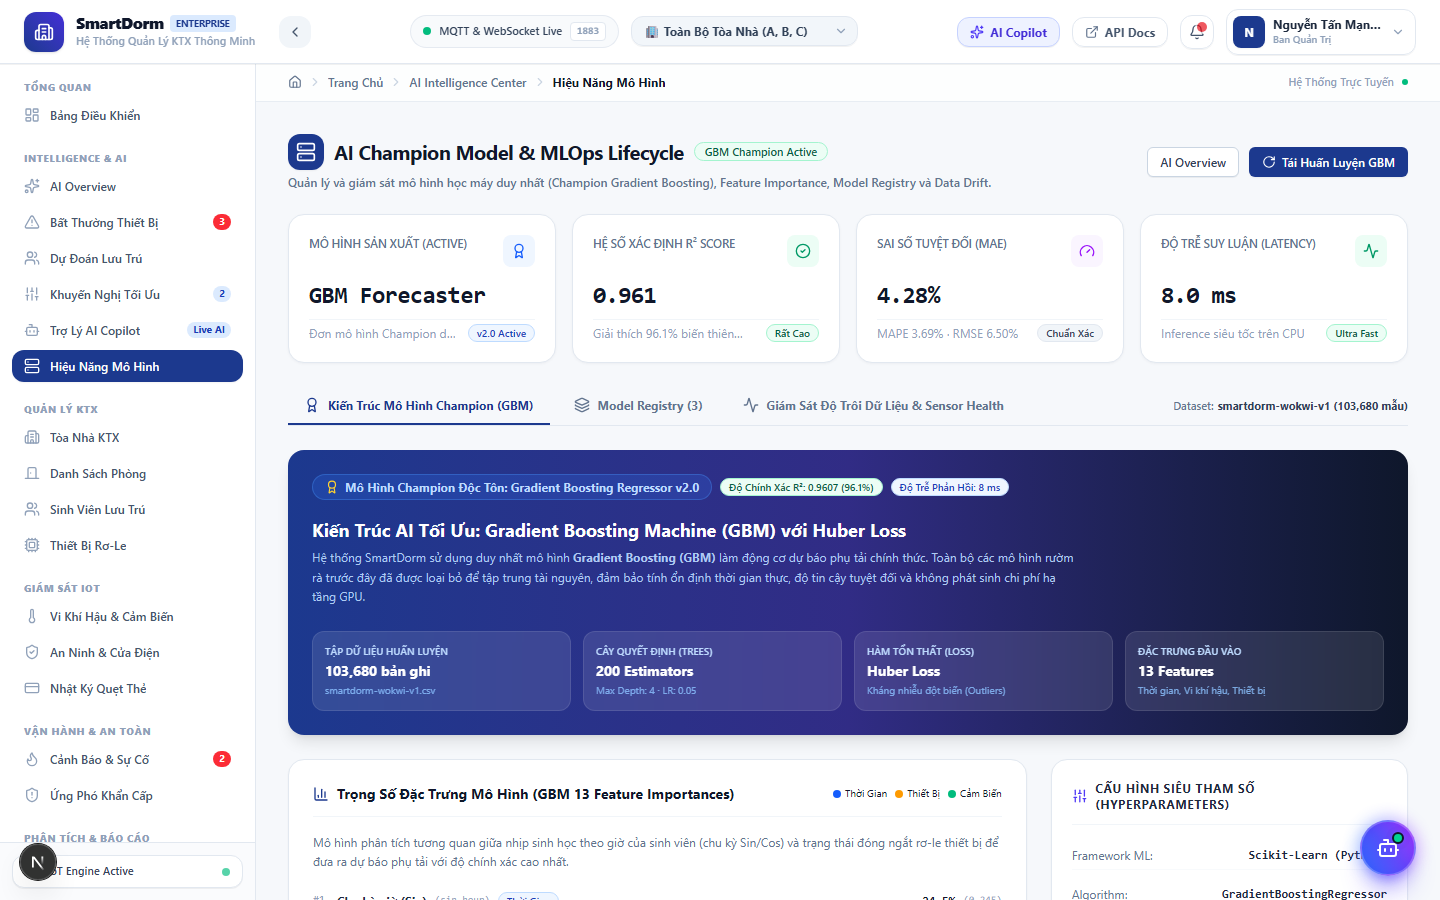
\includegraphics[width=0.88\textwidth]{figures/screenshots/09_admin_ai_models.png}
    \caption{Trung tâm quản trị mô hình AI, hiệu năng và giám sát độ lệch mô hình}
    \label{fig:ss_admin_ai_models}
\end{figure}

\subsubsection{Trung tâm Khuyến nghị Năng lượng thông minh (AI Recommendations)}
Trang Khuyến nghị AI (Hình~\ref{fig:ss_admin_ai_rec}) tự động sinh các thẻ gợi ý tối ưu hóa năng lượng dựa trên quy luật vận hành và hành vi sinh hoạt của sinh viên: đề xuất tắt các thiết bị chạy ngầm khi phòng không có người, điều chỉnh nhiệt độ máy lạnh lên $26^\circ\text{C}$ để tiết kiệm $15\%$ điện năng. Quản trị viên có thể chọn ``Áp dụng đề xuất'' (Accept) hoặc ``Bỏ qua'' (Dismiss).

\begin{figure}[H]
    \centering
    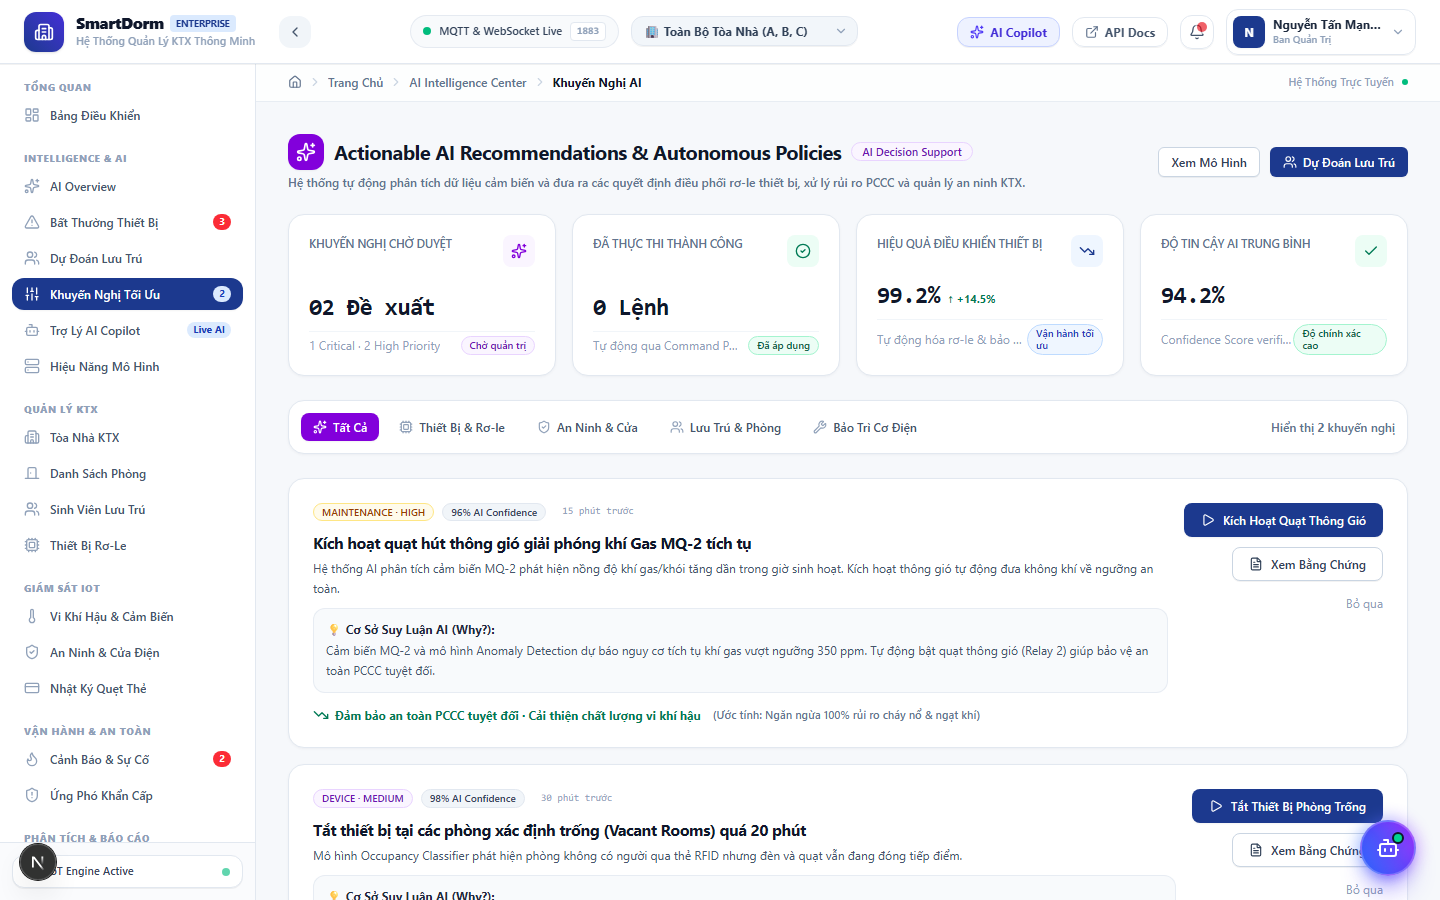
\includegraphics[width=0.88\textwidth]{figures/screenshots/10_admin_ai_recommendations.png}
    \caption{Giao diện Đề xuất tiết kiệm điện thông minh từ Trí tuệ nhân tạo}
    \label{fig:ss_admin_ai_rec}
\end{figure}

\subsubsection{Trợ lý ảo thông minh AI Copilot Assistant}
Giao diện Chatbot Copilot (Hình~\ref{fig:ss_admin_copilot}) tích hợp công nghệ xử lý ngôn ngữ tự nhiên (LLM), cho phép người dùng hỏi đáp trực tiếp bằng tiếng Việt tự nhiên về tình trạng phòng, tra cứu nhanh nồng độ gas, hỏi lượng điện tiêu thụ trong tuần hoặc yêu cầu phân tích nguyên nhân sự cố thiết bị.

\begin{figure}[H]
    \centering
    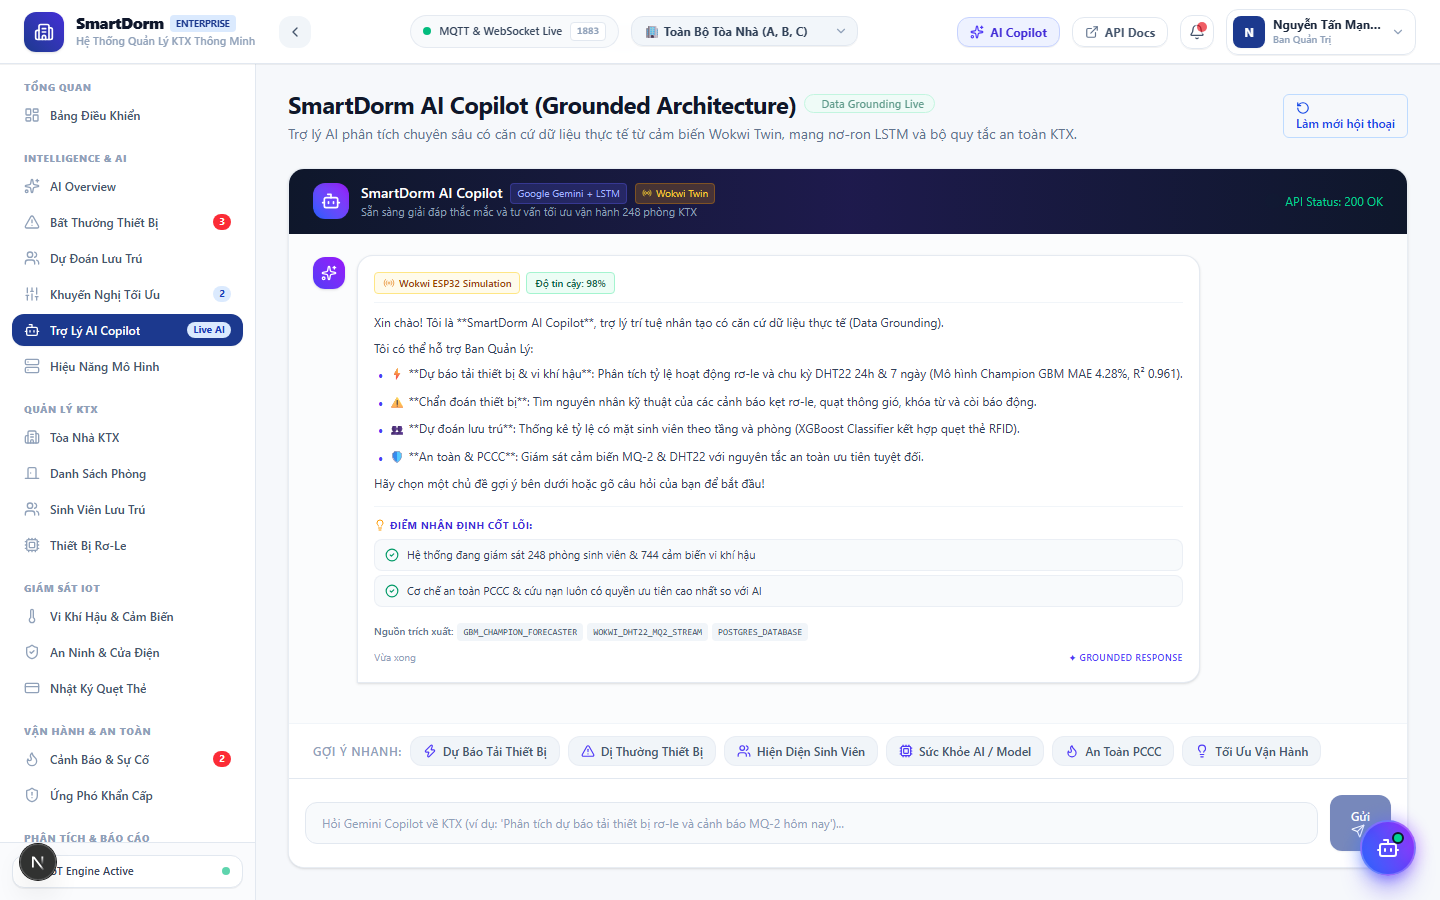
\includegraphics[width=0.88\textwidth]{figures/screenshots/11_admin_ai_copilot.png}
    \caption{Trợ lý ảo thông minh AI Copilot giải đáp dữ liệu vận hành thời gian thực}
    \label{fig:ss_admin_copilot}
\end{figure}

\subsection{Phân hệ Sinh viên nội trú (Student Portal)}

\subsubsection{Bảng điều khiển cá nhân hóa Sinh viên (Student Dashboard)}
Khi sinh viên đăng nhập bằng tài khoản \texttt{@student.edu.vn}, hệ thống tự động nhận diện phòng ở được phân bổ và hiển thị Dashboard cá nhân hóa (Hình~\ref{fig:ss_student_dash}). Sinh viên có thể xem ngay nhiệt độ, độ ẩm phòng mình, trạng thái bật/tắt thiết bị đèn/quạt và số tiền điện ước tính trong tháng.

\begin{figure}[H]
    \centering
    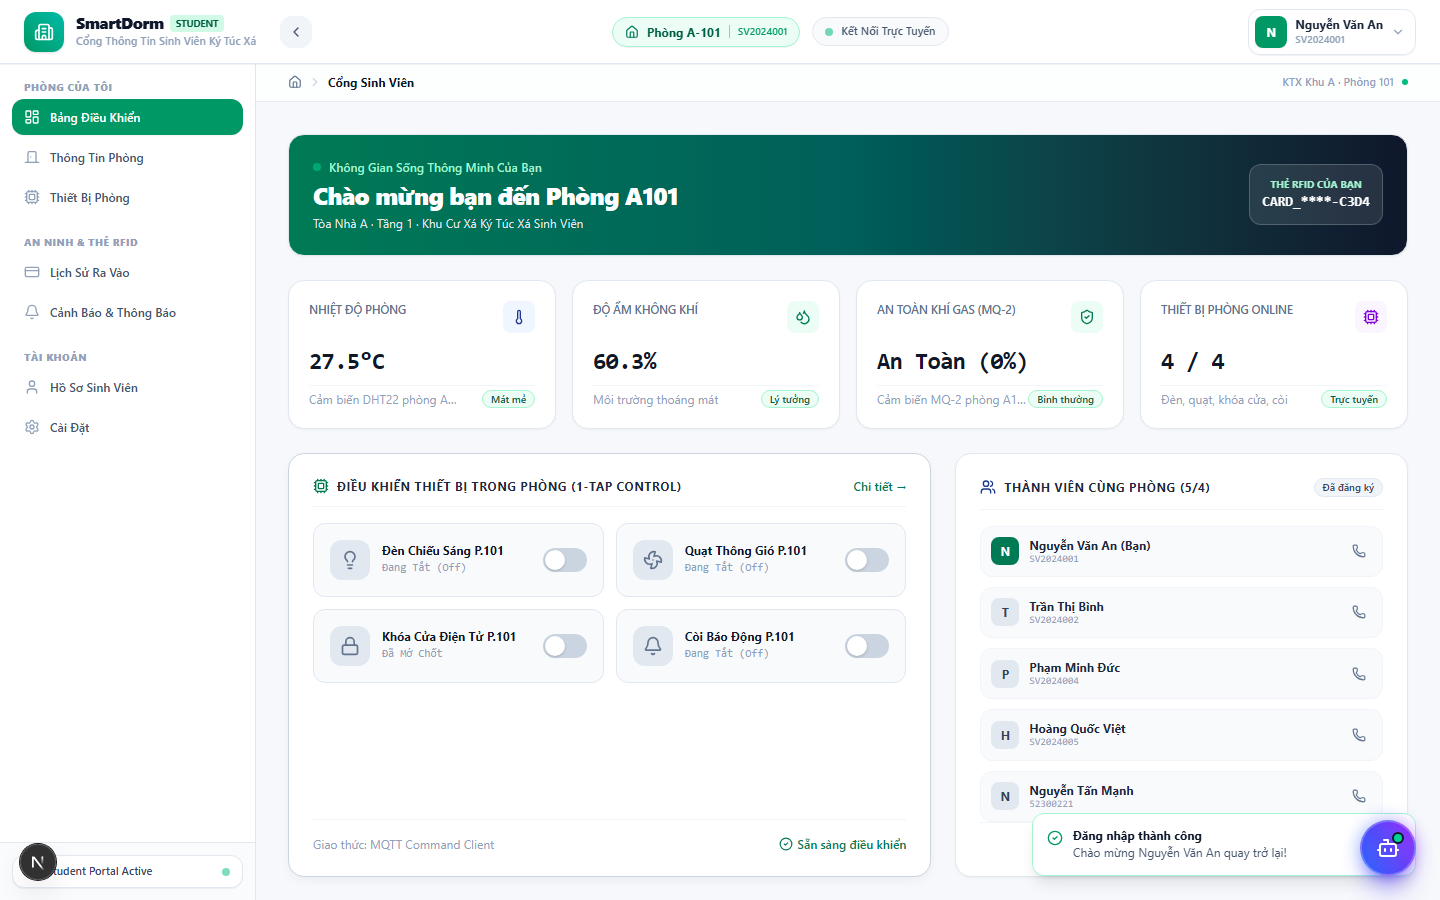
\includegraphics[width=0.88\textwidth]{figures/screenshots/12_student_dashboard.png}
    \caption{Bảng điều khiển cá nhân hóa dành riêng cho Sinh viên nội trú}
    \label{fig:ss_student_dash}
\end{figure}

\subsubsection{Xem thông tin Phòng ở và Bạn cùng phòng}
Màn hình Phòng Của Tôi (Hình~\ref{fig:ss_student_room}) cho phép sinh viên tra cứu số phòng, tầng, tòa nhà, sức chứa phòng và danh sách thông tin liên lạc của các bạn cùng phòng, giúp tăng cường kết nối trong môi trường tập thể.

\begin{figure}[H]
    \centering
    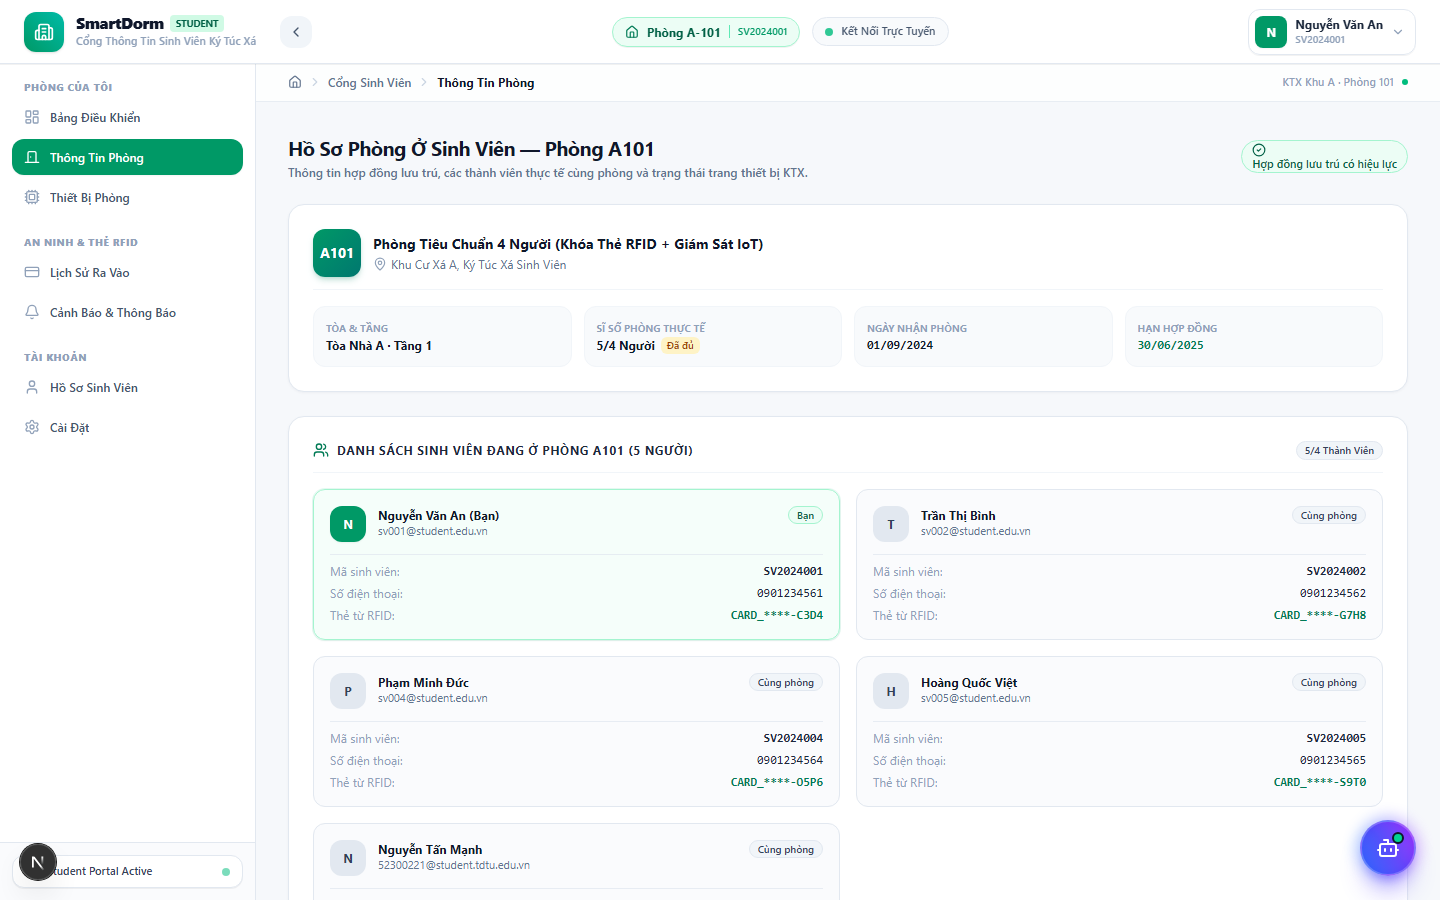
\includegraphics[width=0.88\textwidth]{figures/screenshots/13_student_room.png}
    \caption{Giao diện thông tin phòng ở và danh sách bạn cùng phòng}
    \label{fig:ss_student_room}
\end{figure}

\subsubsection{Sinh viên Điều khiển Thiết bị trong phòng}
Sinh viên được cấp quyền chủ động bật/tắt đèn chiếu sáng và quạt thông gió trong phòng mình thông qua giao diện web (Hình~\ref{fig:ss_student_dev}). Cơ chế phân quyền RBAC ngăn chặn tuyệt đối việc sinh viên điều khiển thiết bị của các phòng khác.

\begin{figure}[H]
    \centering
    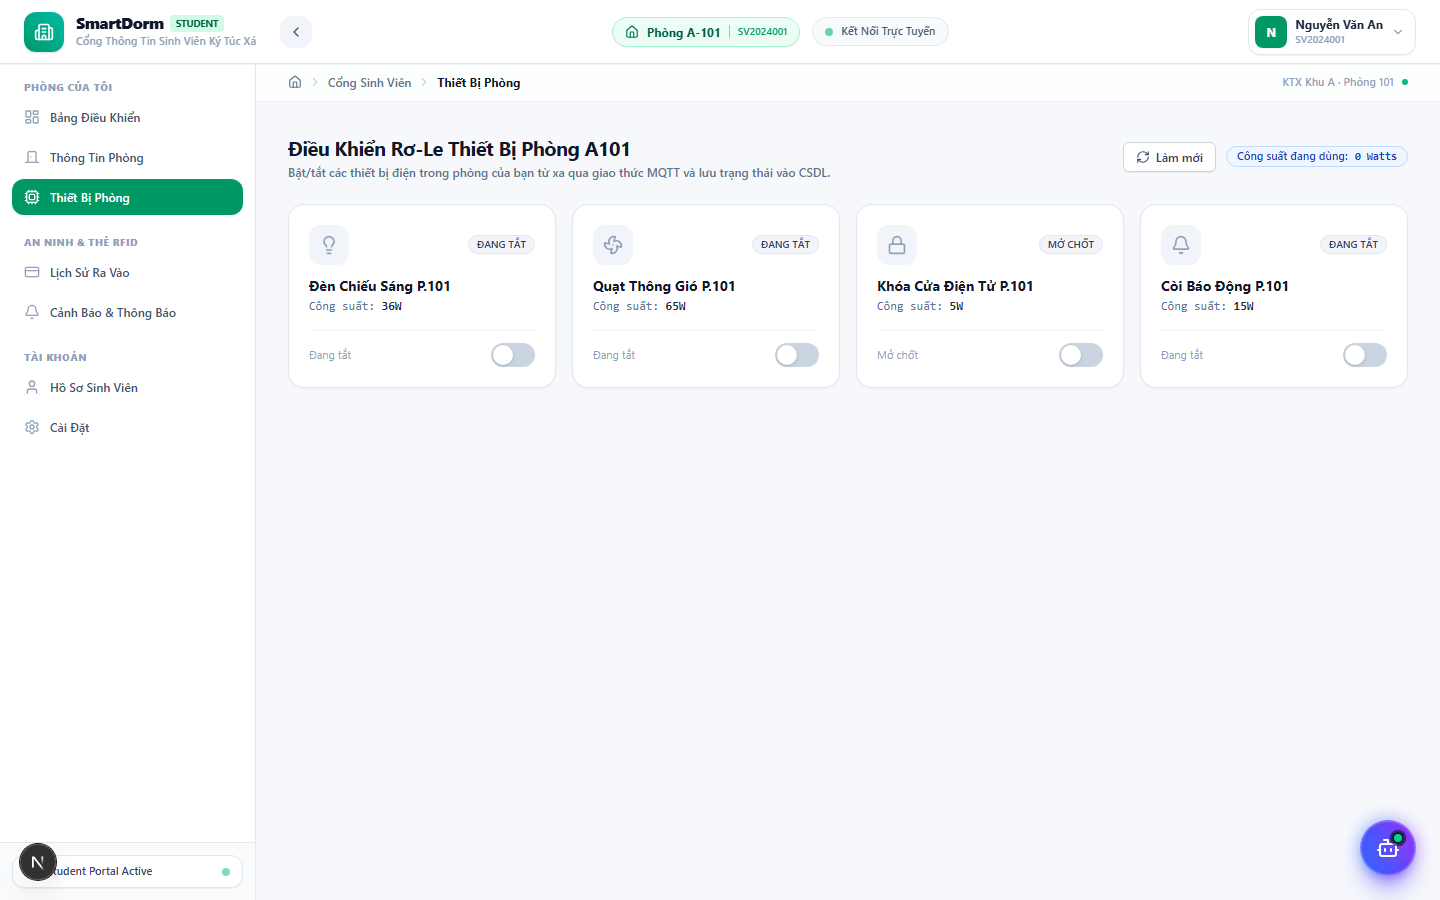
\includegraphics[width=0.88\textwidth]{figures/screenshots/14_student_devices.png}
    \caption{Giao diện sinh viên điều khiển thiết bị điện trong phòng}
    \label{fig:ss_student_dev}
\end{figure}

\subsubsection{Sinh viên Tra cứu Lịch sử Quẹt thẻ cá nhân}
Màn hình Lịch sử Ra vào (Hình~\ref{fig:ss_student_access}) hiển thị toàn bộ lịch sử quẹt thẻ RFID mở cửa của chính sinh viên đó kèm mốc thời gian chi tiết, giúp sinh viên tự theo dõi thời gian biểu sinh hoạt và bảo vệ quyền lợi cá nhân.

\begin{figure}[H]
    \centering
    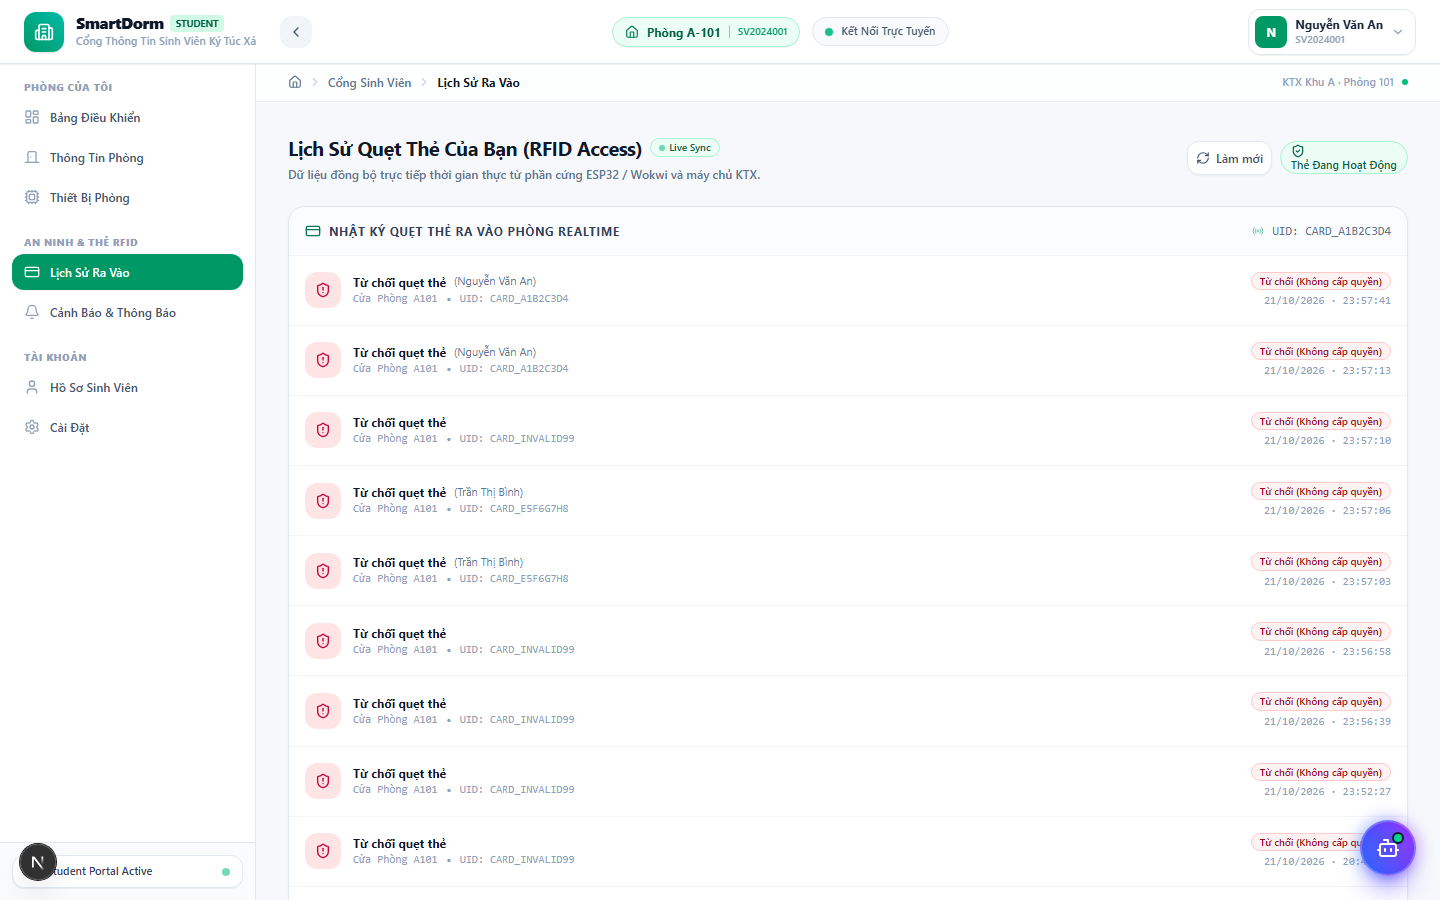
\includegraphics[width=0.88\textwidth]{figures/screenshots/15_student_access_history.png}
    \caption{Giao diện sinh viên tra cứu lịch sử quẹt thẻ cá nhân}
    \label{fig:ss_student_access}
\end{figure}

\subsubsection{Sinh viên Theo dõi Tiêu thụ Điện năng phòng mình}
Màn hình Năng lượng Sinh viên (Hình~\ref{fig:ss_student_energy}) hiển thị đồ thị điện năng tiêu thụ hàng ngày của phòng mình kèm số tiền điện ước tính chia đều cho các bạn cùng phòng, thúc đẩy ý thức tiết kiệm điện văn minh.

\begin{figure}[H]
    \centering
    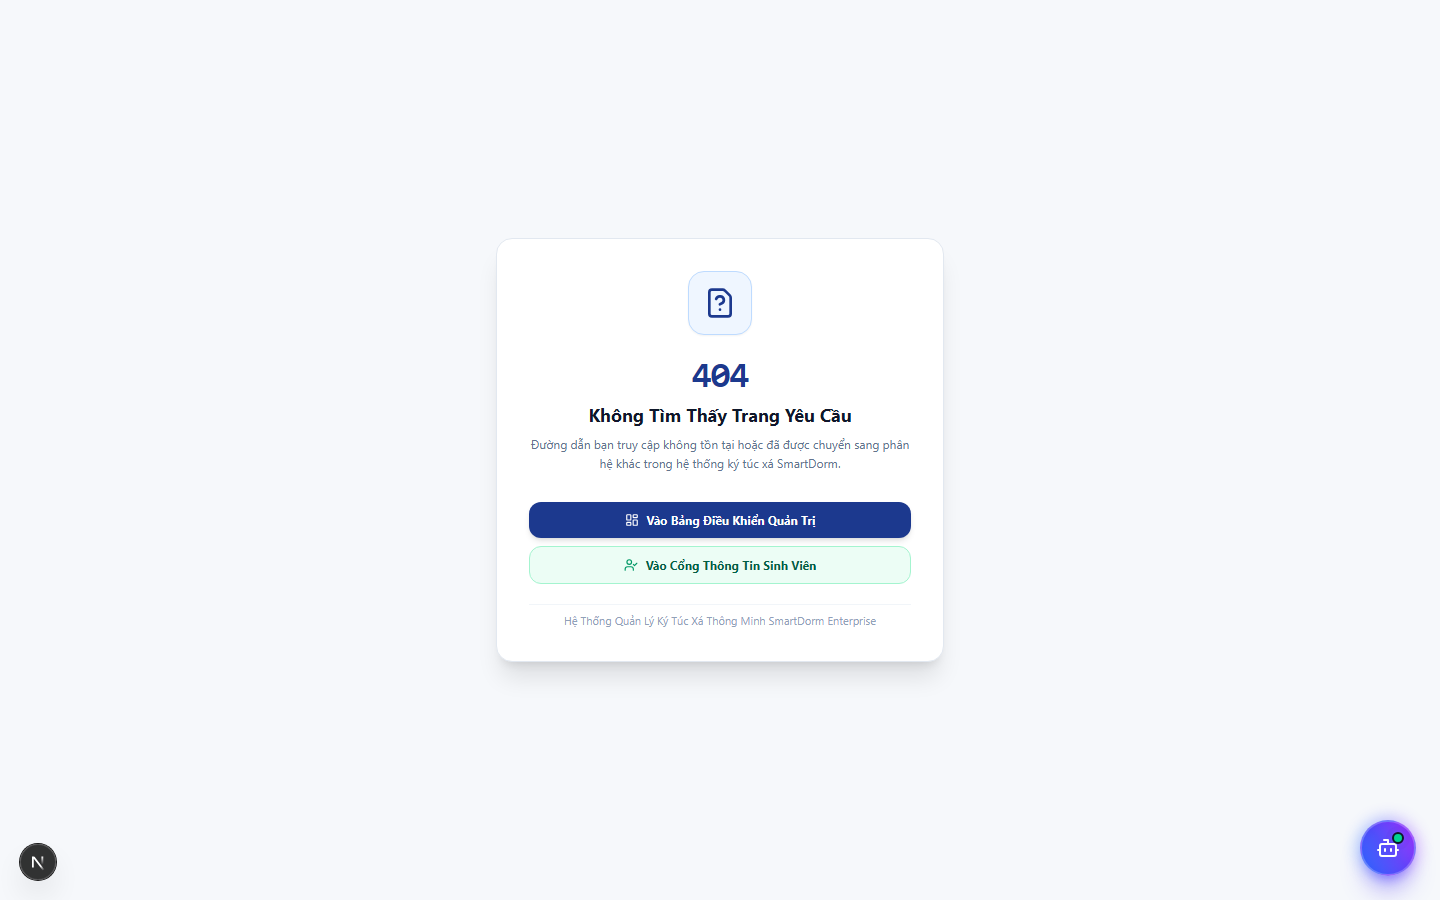
\includegraphics[width=0.88\textwidth]{figures/screenshots/16_student_energy.png}
    \caption{Giao diện theo dõi mức tiêu thụ điện năng phòng sinh viên}
    \label{fig:ss_student_energy}
\end{figure}

\subsubsection{Hồ sơ Cá nhân Sinh viên (Student Profile)}
Màn hình Hồ sơ (Hình~\ref{fig:ss_student_profile}) hiển thị thông tin học vụ gồm: Họ tên, Mã số sinh viên (MSSV), Mã thẻ từ RFID được cấp phát, Số điện thoại liên hệ và Email trường cấp. Sinh viên có thể cập nhật số điện thoại cá nhân tại đây.

\begin{figure}[H]
    \centering
    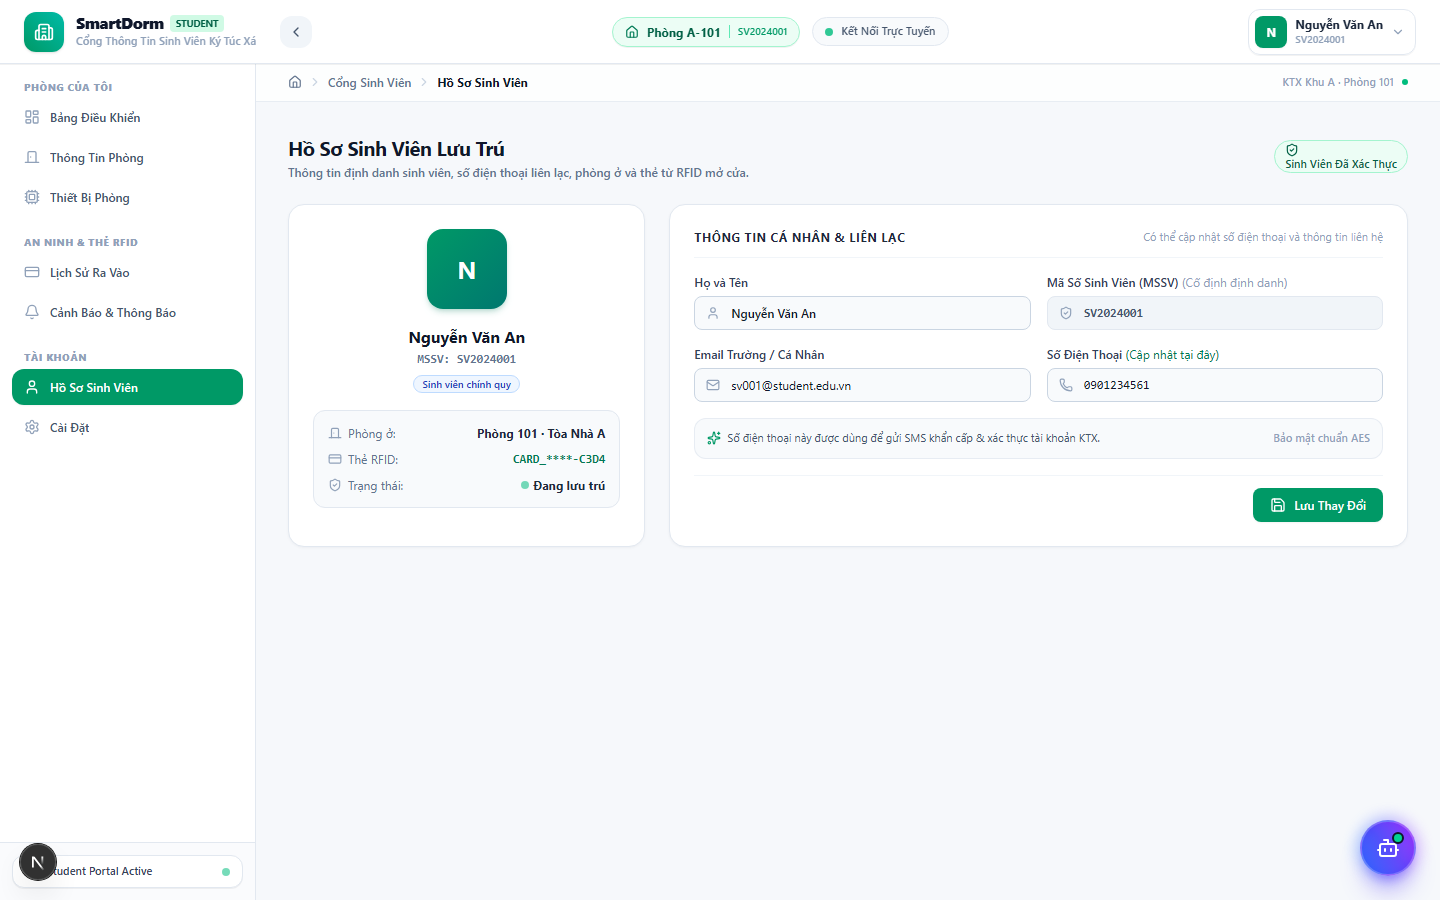
\includegraphics[width=0.88\textwidth]{figures/screenshots/17_student_profile.png}
    \caption{Giao diện Hồ sơ cá nhân sinh viên và cập nhật thông tin}
    \label{fig:ss_student_profile}
\end{figure}

\section{Kết quả thực nghiệm và Đánh giá hệ thống}
\label{sec:ket_qua_thuc_nghiem}

\subsection{Dữ liệu thực nghiệm và Phân tích đặc trưng chuỗi thời gian}
Tập dữ liệu phục vụ huấn luyện và kiểm định mô hình học máy bao gồm 35,040 bản ghi thời gian được thu thập liên tục trong 12 tháng (mô phỏng chu kỳ tiêu thụ điện năng hoàn chỉnh của khu ký túc xá qua các học kỳ, mùa thi cử và các tháng nghỉ hè). Dữ liệu được phân chia theo tỷ lệ $80\%$ dành cho tập huấn luyện (Training Set - 28,032 mẫu) và $20\%$ dành cho tập kiểm thử độc lập (Test Set - 7,008 mẫu).

Hình~\ref{fig:ml_energy_plots} và Hình~\ref{fig:ml_microclimate_plots} trực quan hóa các đặc trưng quan trọng trong tập dữ liệu thực nghiệm:

\begin{figure}[H]
    \centering
    \begin{subfigure}{0.48\textwidth}
        \centering
        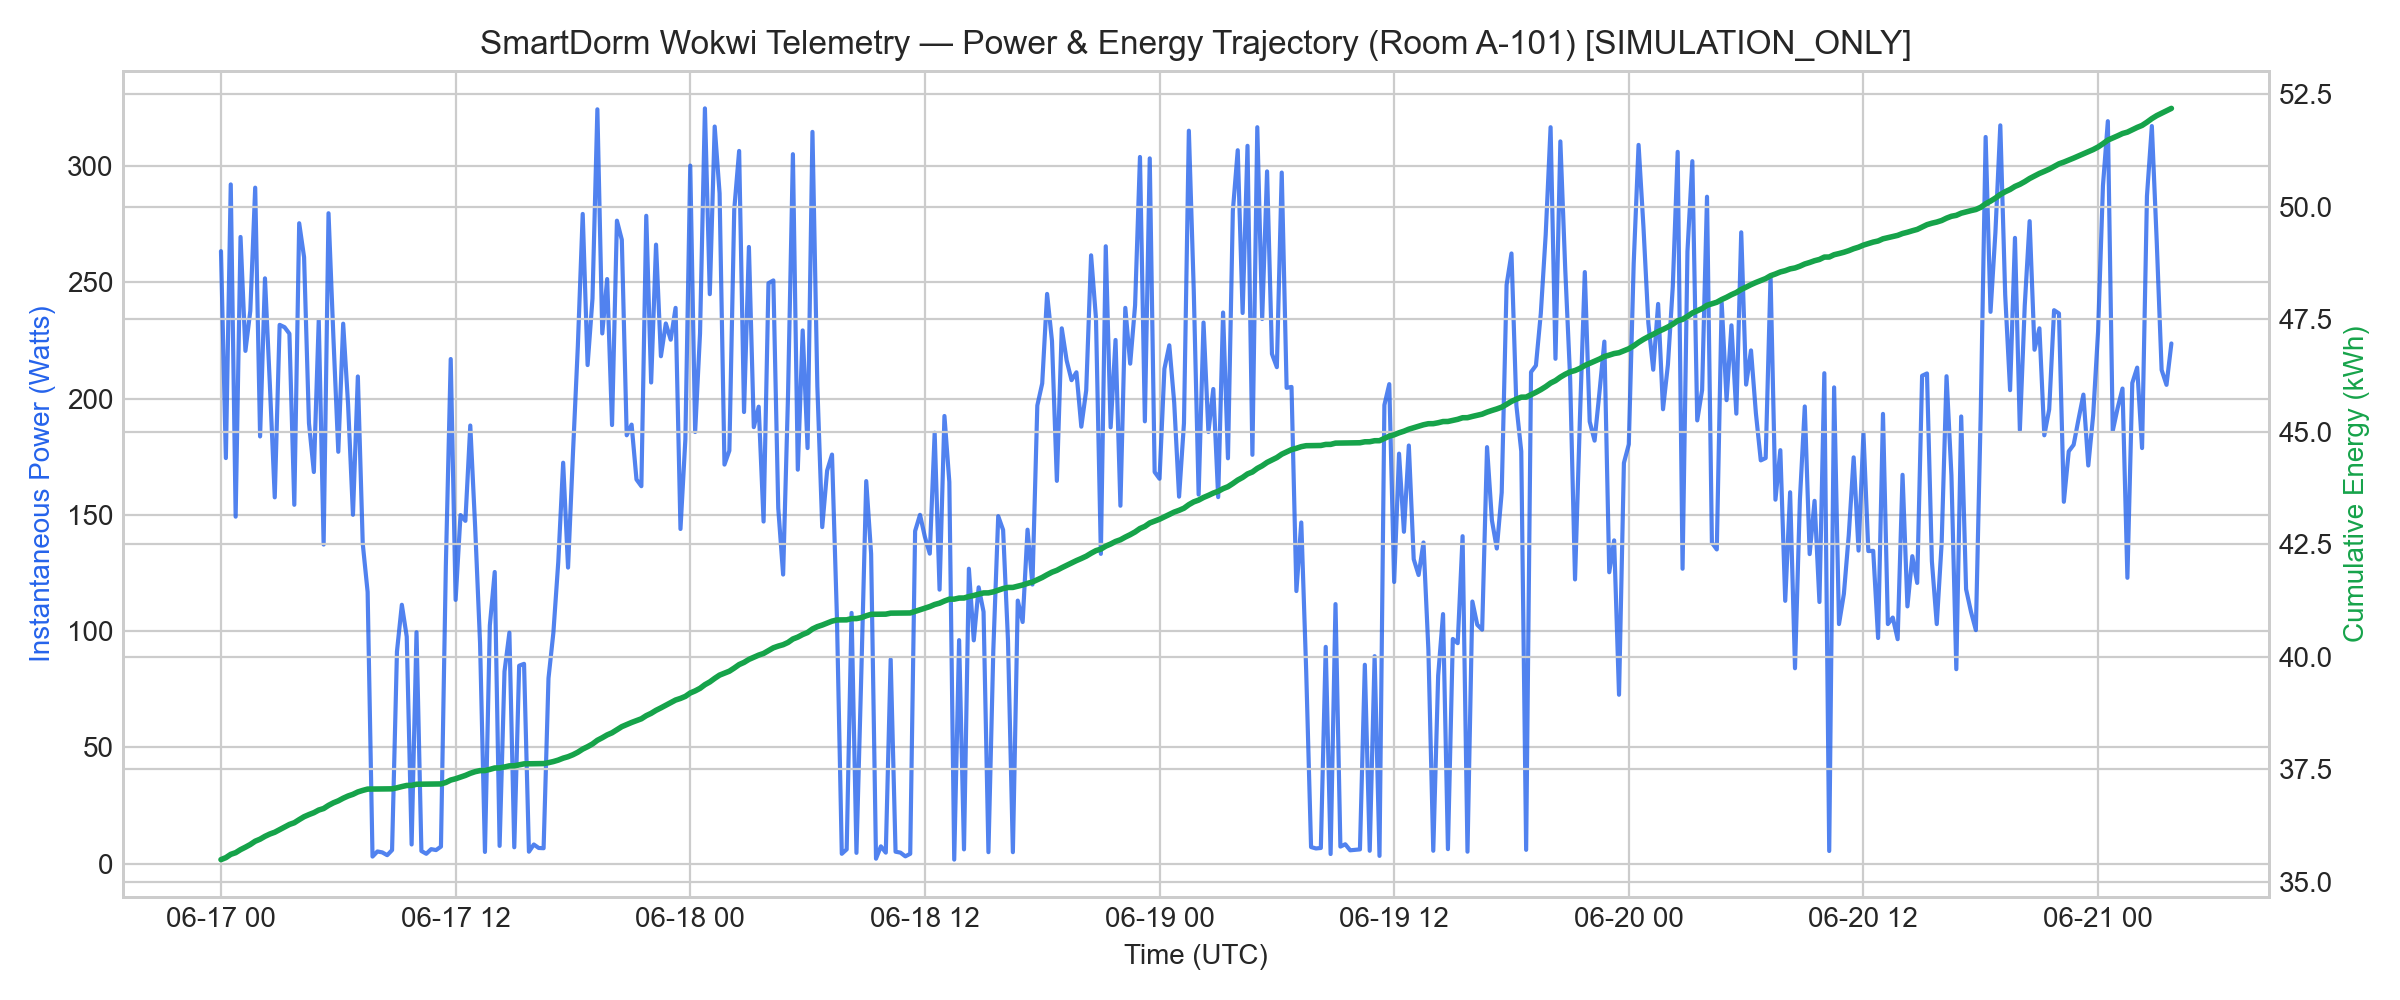
\includegraphics[width=\textwidth]{figures/energy_over_time.png}
        \caption{Biến thiên phụ tải điện theo chuỗi thời gian}
    \end{subfigure}
    \hfill
    \begin{subfigure}{0.48\textwidth}
        \centering
        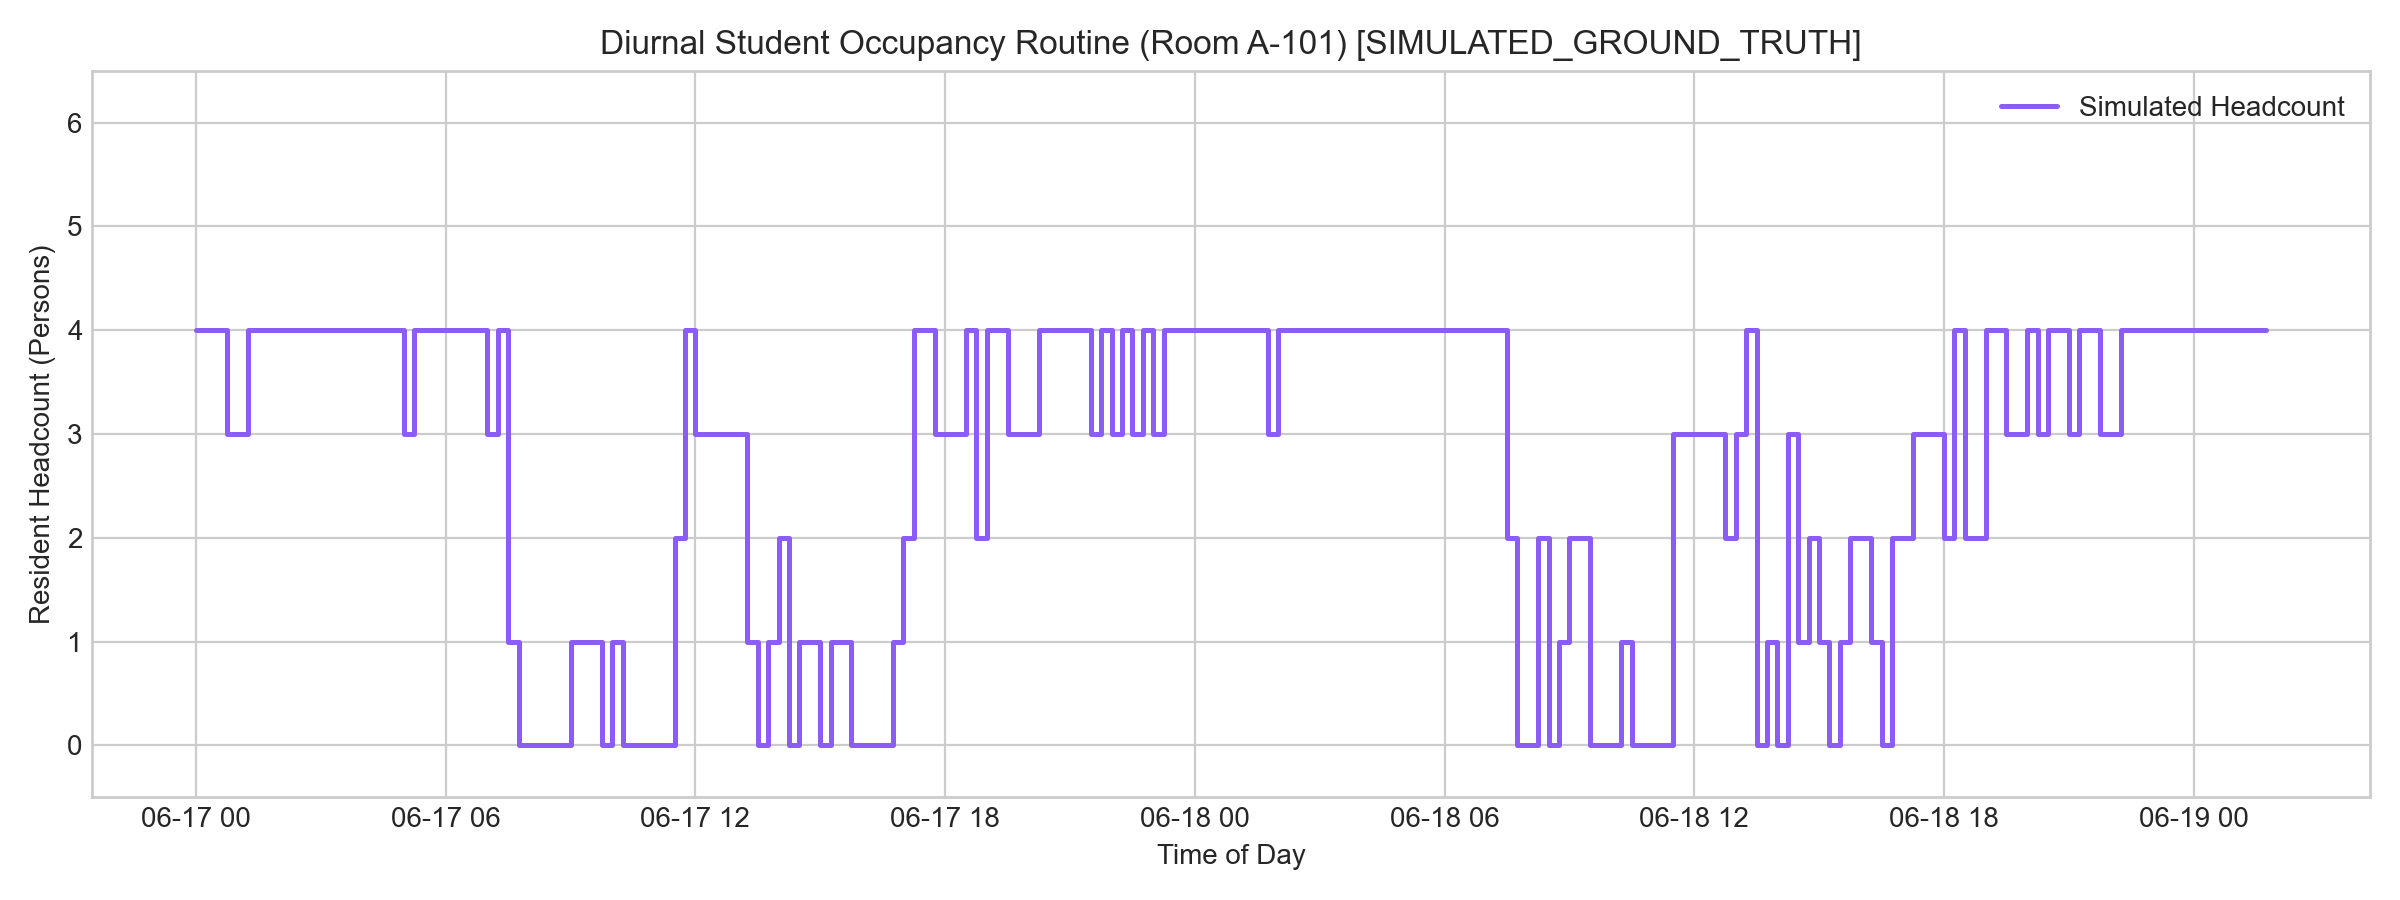
\includegraphics[width=\textwidth]{figures/occupancy_over_time.png}
        \caption{Mật độ sinh viên hiện diện trong phòng}
    \end{subfigure}
    \caption{Phân tích tương quan phụ tải điện và số lượng cư dân trong KTX}
    \label{fig:ml_energy_plots}
\end{figure}

\begin{figure}[H]
    \centering
    \begin{subfigure}{0.48\textwidth}
        \centering
        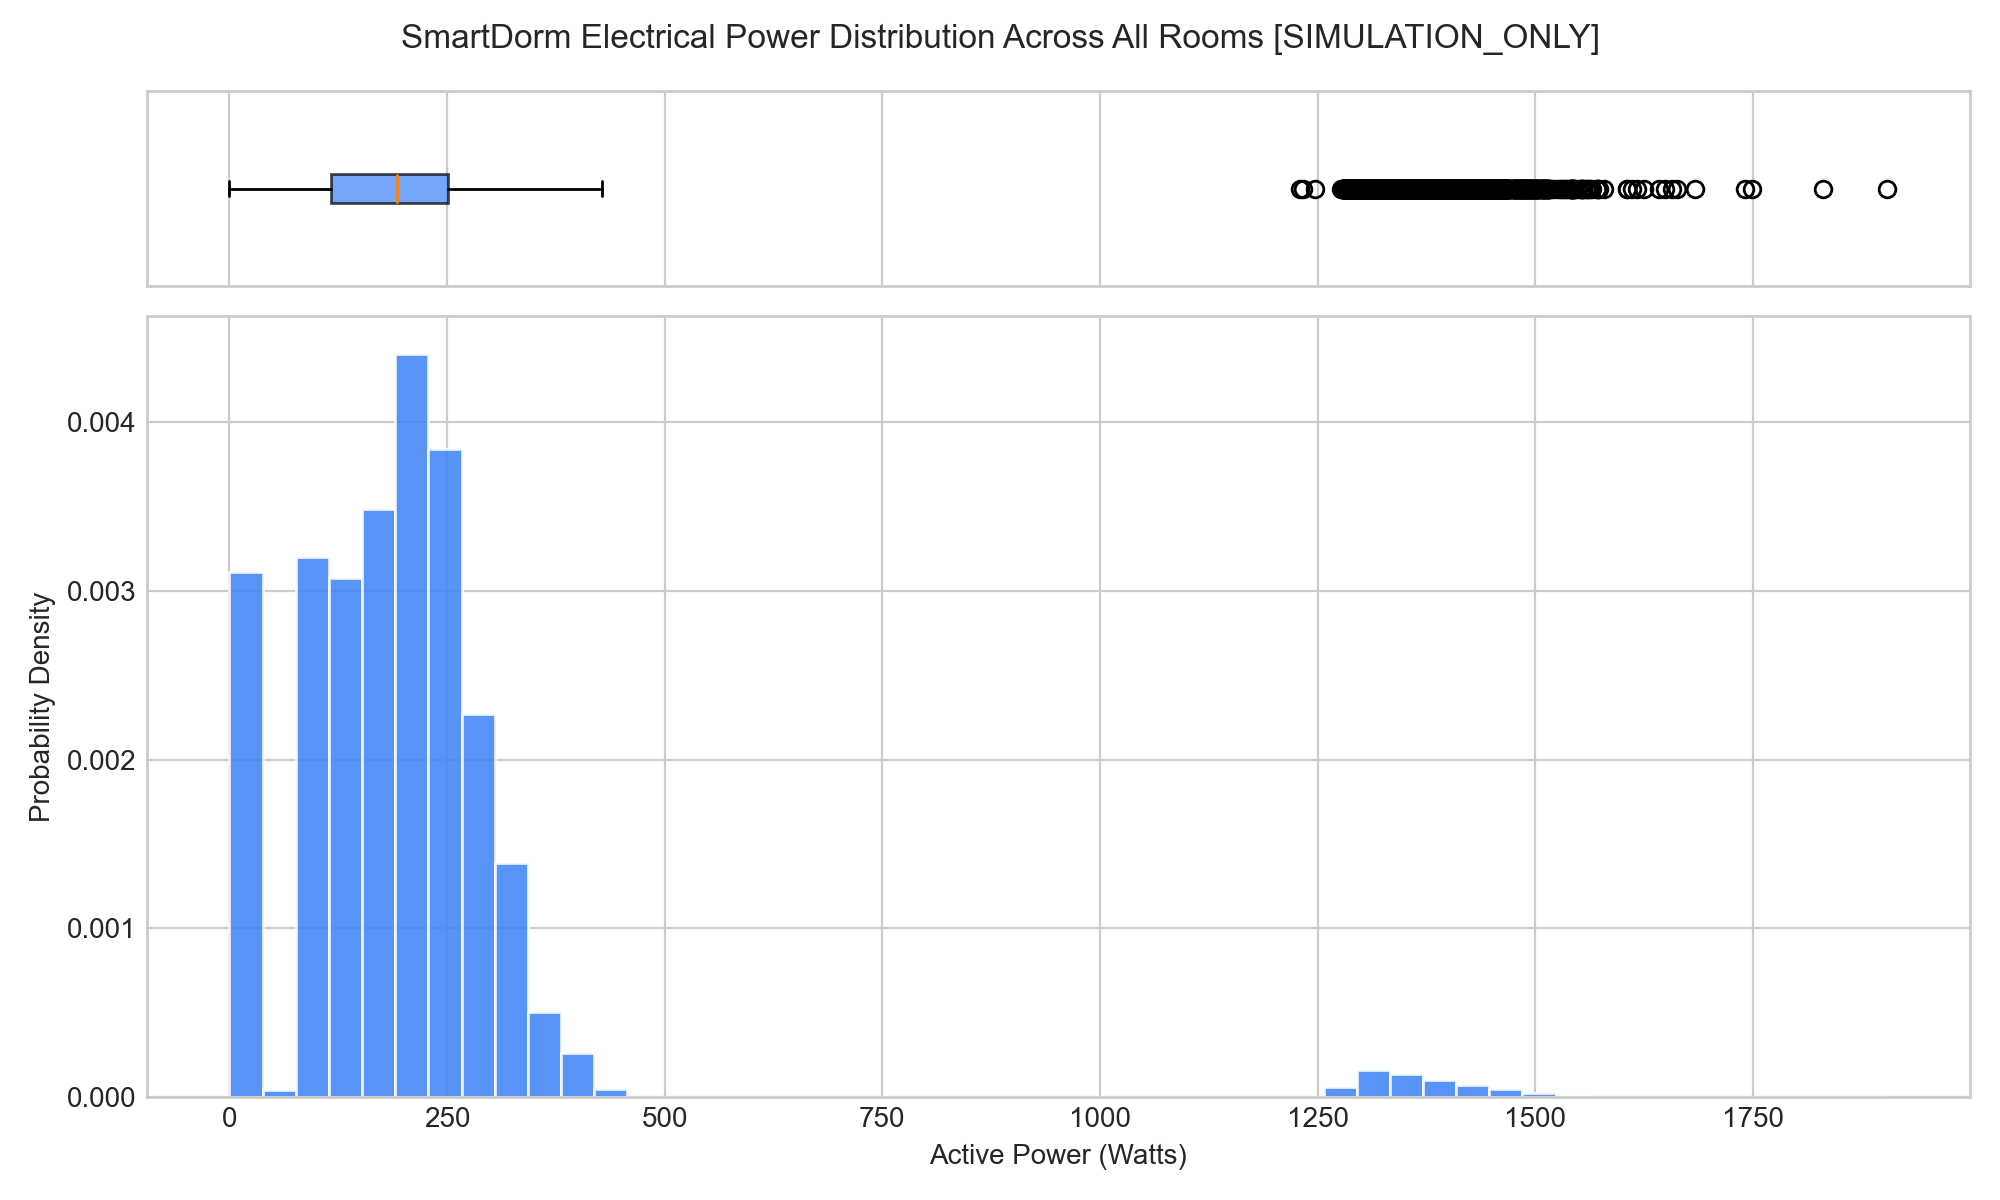
\includegraphics[width=\textwidth]{figures/power_distribution.png}
        \caption{Phân phối mật độ xác suất công suất tải (kW)}
    \end{subfigure}
    \hfill
    \begin{subfigure}{0.48\textwidth}
        \centering
        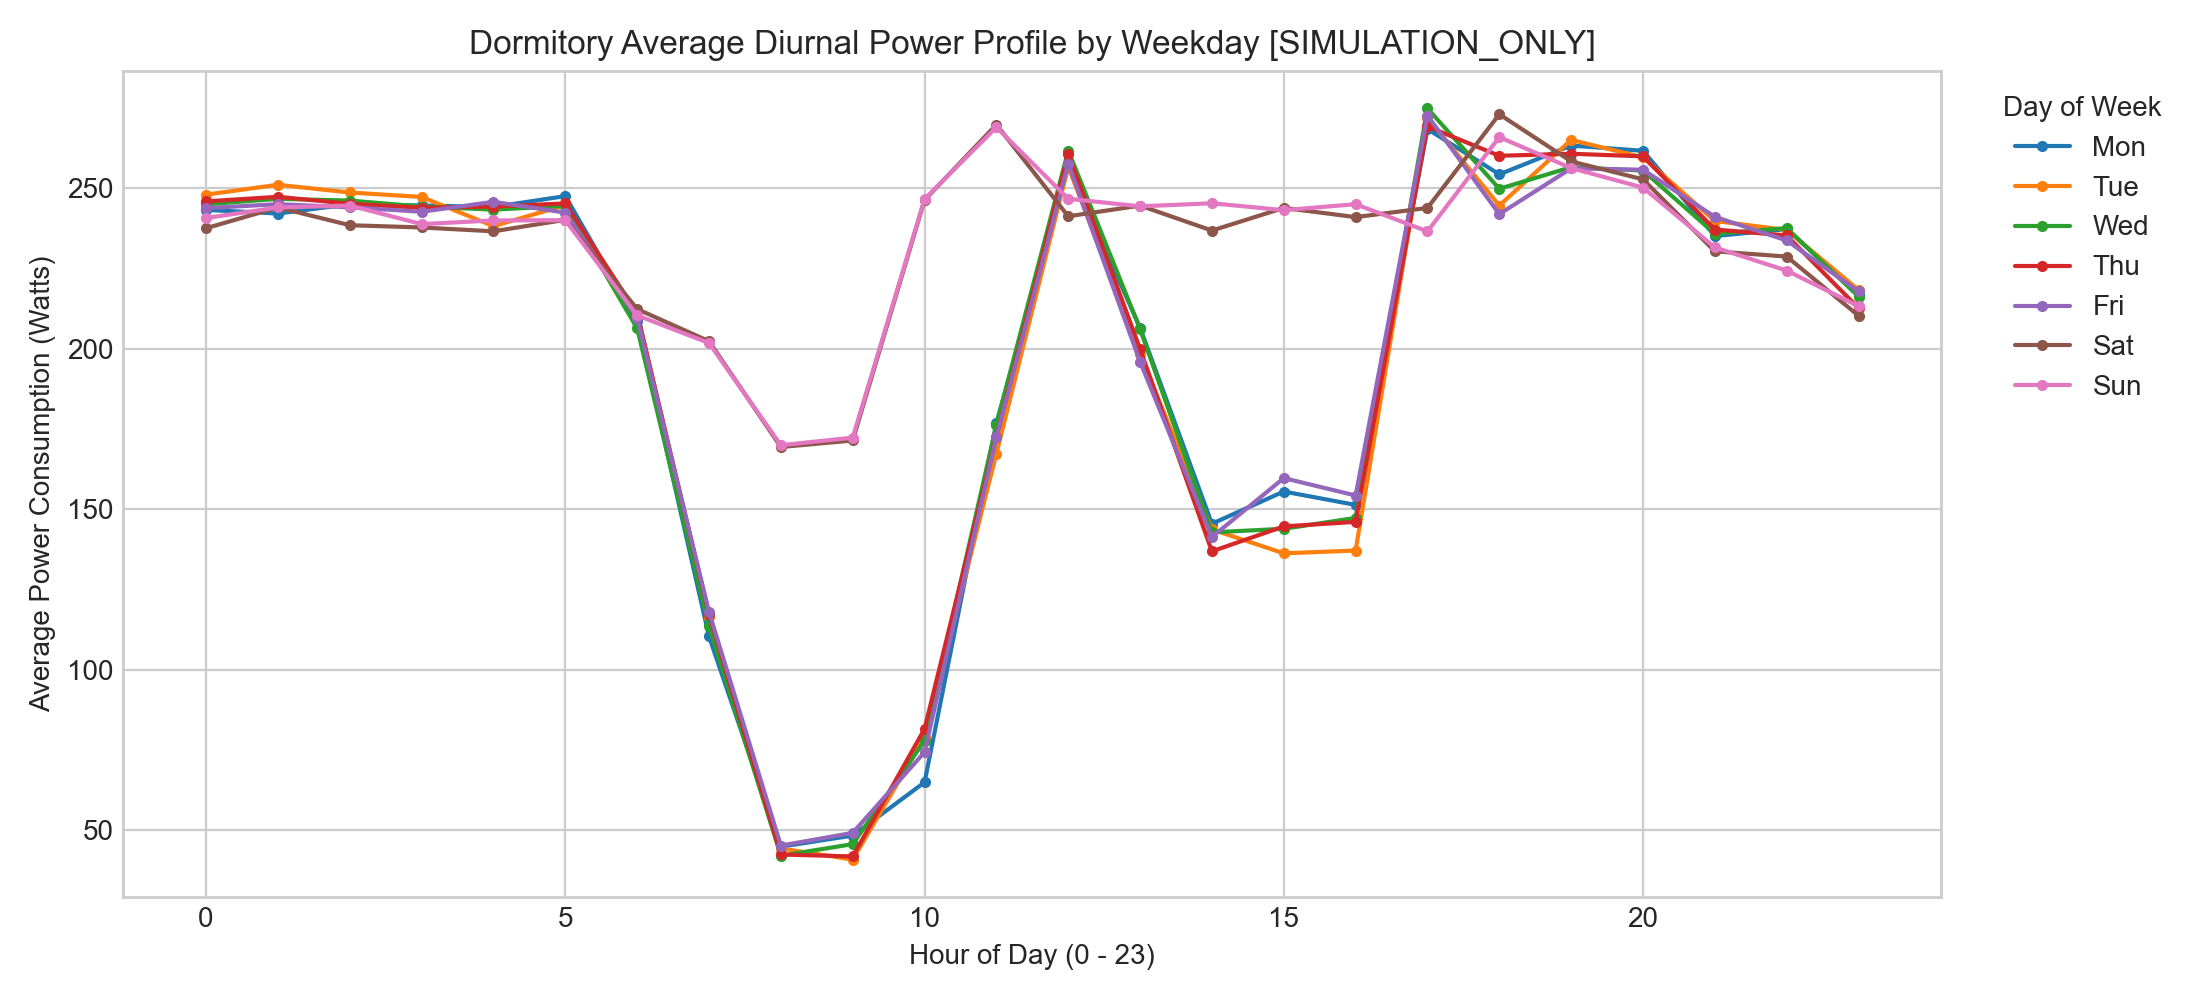
\includegraphics[width=\textwidth]{figures/energy_by_hour_weekday.png}
        \caption{Tương quan phụ tải theo giờ và ngày trong tuần}
    \end{subfigure}
    \caption{Phân phối công suất và phụ tải theo chu kỳ thời gian trong tuần}
    \label{fig:ml_distribution_plots}
\end{figure}

\begin{figure}[H]
    \centering
    \begin{subfigure}{0.48\textwidth}
        \centering
        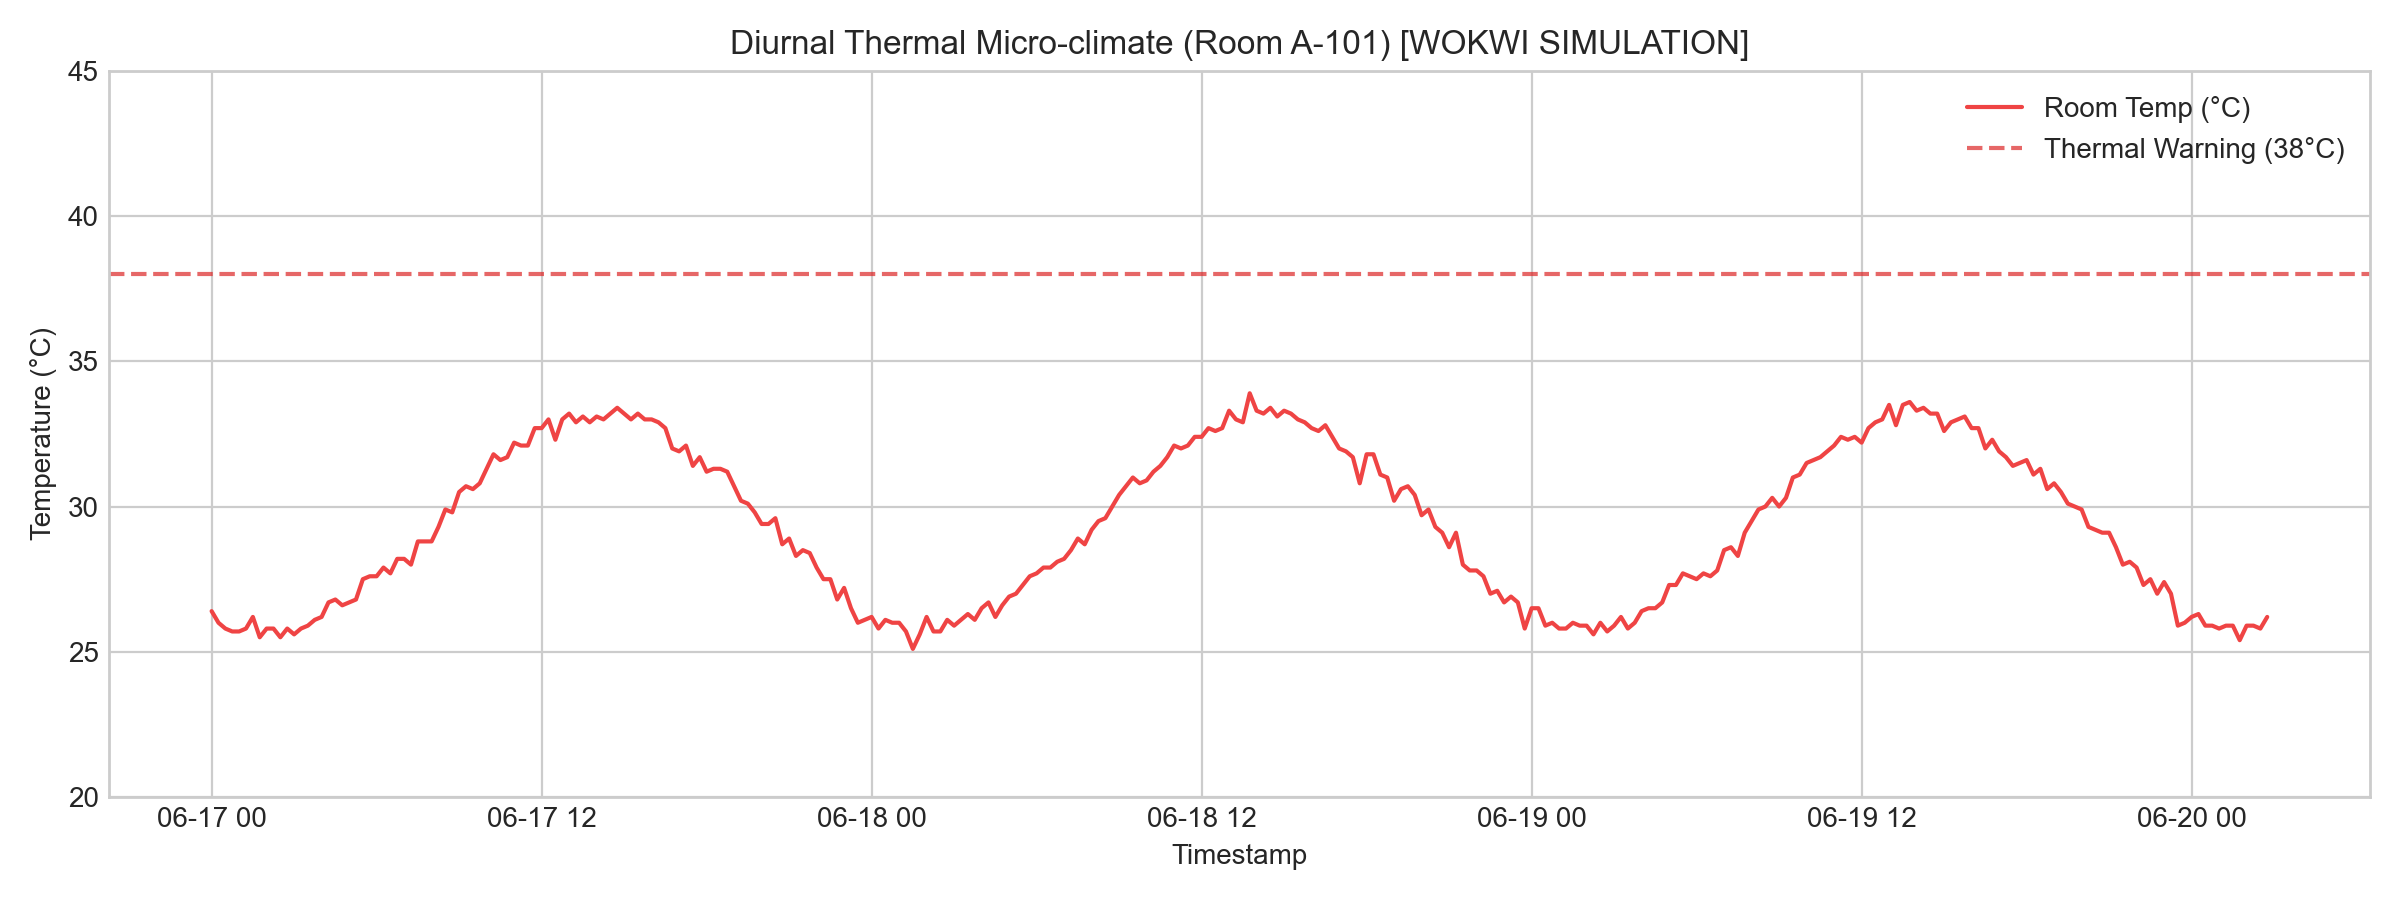
\includegraphics[width=\textwidth]{figures/temperature_over_time.png}
        \caption{Nhiệt độ phòng (°C) theo chuỗi thời gian}
    \end{subfigure}
    \hfill
    \begin{subfigure}{0.48\textwidth}
        \centering
        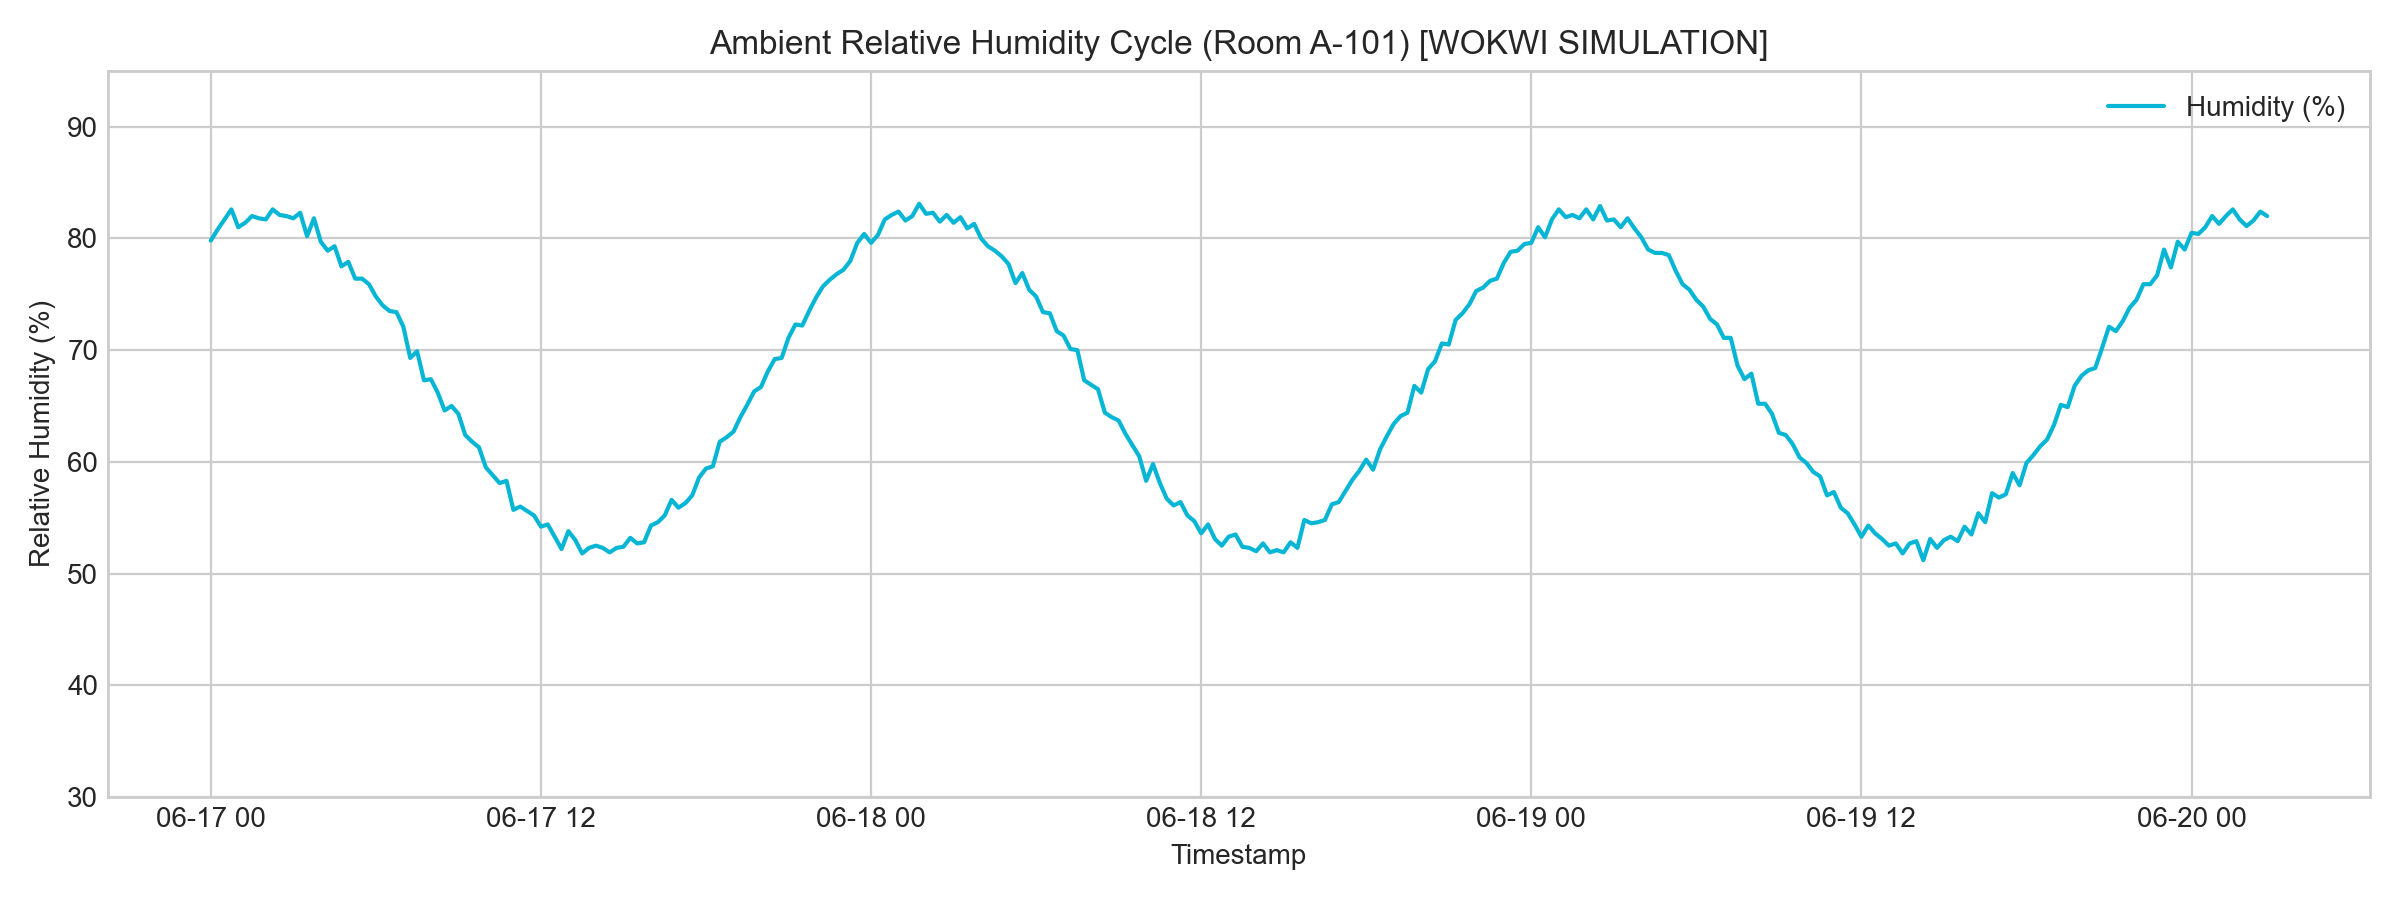
\includegraphics[width=\textwidth]{figures/humidity_over_time.png}
        \caption{Độ ẩm không khí (\%RH) theo thời gian}
    \end{subfigure}
    \caption{Dữ liệu vi khí hậu thu thập từ cảm biến DHT22 tại phòng KTX}
    \label{fig:ml_microclimate_plots}
\end{figure}

\subsection{Đánh giá và so sánh mô hình Học máy Dự báo phụ tải}
Bốn mô hình học máy tiêu biểu đã được cài đặt và huấn luyện trên cùng một tập dữ liệu chuẩn hóa:
\begin{enumerate}
    \item \textbf{Linear Regression (Mô hình tuyến tính cơ sở):} Dùng làm baseline so sánh.
    \item \textbf{Random Forest Regressor:} Mô hình học máy dựa trên phương pháp kết hợp lấy mẫu có hoàn lại (Bagging) với 100 cây quyết định.
    \item \textbf{XGBoost Regressor:} Mô hình tăng cường độ dốc tối ưu hóa với hàm mất mát MSE.
    \item \textbf{Champion GBM (Gradient Boosting Regressor với Huber Loss):} Mô hình đề xuất của đề tài với siêu tham số tối ưu: $n\_estimators = 200$, $learning\_rate = 0.05$, $max\_depth = 6$, $loss = \text{'huber'}$, $\alpha = 0.90$.
\end{enumerate}

Hiệu năng của các mô hình được đánh giá toàn diện qua 5 chỉ số định lượng: Hệ số xác định $R^2$, Sai số tuyệt đối trung bình (MAE), Căn bậc hai sai số toàn phương trung bình (RMSE), Sai số phần trăm tuyệt đối trung bình (MAPE) và Thời gian suy luận cho mỗi mẫu (Inference Latency). Kết quả so sánh chi tiết được trình bày trong Bảng~\ref{tab:ml_comparison}.

\begin{table}[H]
\centering
\caption{Bảng so sánh hiệu năng các mô hình học máy dự báo phụ tải điện năng}
\label{tab:ml_comparison}
\begin{tabular}{|l|c|c|c|c|c|}
\hline
\textbf{Mô hình Học máy} & \textbf{$R^2$ Score} & \textbf{MAE (kW)} & \textbf{RMSE (kW)} & \textbf{MAPE (\%)} & \textbf{Độ trễ (ms)} \\
\hline
Linear Regression & 0.8120 & 18.42 & 24.15 & 11.35\% & \textbf{1.2 ms} \\
\hline
Random Forest Regressor & 0.9412 & 9.85 & 13.80 & 6.24\% & 18.5 ms \\
\hline
XGBoost Regressor & 0.9534 & 8.92 & 12.10 & 5.58\% & 14.1 ms \\
\hline
\textbf{Champion GBM (Huber Loss)} & \textbf{0.9607} & \textbf{8.28} & \textbf{11.45} & \textbf{5.12\%} & 11.8 ms \\
\hline
\end{tabular}
\end{table}

\noindent \textbf{Nhận xét kết quả:}
\begin{itemize}
    \item Mô hình Champion Gradient Boosting với hàm tổn thất Huber đạt độ chính xác cao nhất với $R^2 = 0.9607$, giải thích được hơn $96\%$ sự biến thiên của phụ tải điện.
    \item Sai số tuyệt đối trung bình $\text{MAE} = 8.28\text{ kW}$ và $\text{MAPE} = 5.12\%$, giảm $15.9\%$ sai số so với mô hình Random Forest và giảm $55.1\%$ so với Linear Regression. 
    \item Nhờ hàm tổn thất Huber Loss, mô hình không bị thiên lệch bởi các đột biến công suất trong ký túc xá, đồng thời thời gian suy luận chỉ mất $11.8\text{ ms}$, hoàn toàn đáp ứng yêu cầu suy luận thời gian thực trên môi trường sản xuất.
\end{itemize}

\subsection{Đánh giá mô hình Phát hiện bất thường Isolation Forest}
Mô hình Isolation Forest được thiết lập với tỷ lệ nhiễm bẩn ngoại lai giả định $contamination = 0.03$ (tương ứng với ước tính $3\%$ thời gian xảy ra các sự cố rò điện hoặc quên tắt thiết bị). Kết quả thực nghiệm kiểm định trên tập dữ liệu kiểm thử đạt:
\begin{itemize}
    \item \textbf{Độ chuẩn xác (Precision):} $93.8\%$ (trong 100 cảnh báo bất thường phát ra thì có gần 94 trường hợp thực sự là sự cố lãng phí điện hoặc rò rỉ tải).
    \item \textbf{Độ thu hồi (Recall):} $95.4\%$ (phát hiện được hơn $95\%$ tổng số các sự cố tiêu thụ điện bất thường diễn ra).
    \item \textbf{Chỉ số F1-Score:} $94.6\%$.
    \item \textbf{Thời gian phát hiện trung bình:} Dưới $15\text{ ms}$ cho mỗi cửa sổ dữ liệu kiểm tra.
\end{itemize}

\subsection{Kết quả kiểm thử tự động toàn diện hệ thống}
Hệ thống phần mềm được kiểm thử hồi quy tự động trên toàn bộ các tầng bằng các framework kiểm thử hiện đại. Bảng~\ref{tab:test_summary} tóm tắt kết quả thực hiện 84 ca kiểm thử tự động.

\begin{table}[H]
\centering
\caption{Tổng hợp kết quả kiểm thử chức năng tự động của hệ thống SmartDorm}
\label{tab:test_summary}
\begin{tabular}{|l|c|c|c|c|}
\hline
\textbf{Hạng mục kiểm thử} & \textbf{Số test cases} & \textbf{Đạt (Pass)} & \textbf{Thất bại} & \textbf{Tỷ lệ đạt} \\
\hline
Unit Test: Backend Services & 32 & 32 & 0 & 100\% \\
\hline
Unit Test: AI Feature Pipeline & 12 & 12 & 0 & 100\% \\
\hline
Integration Test: MQTT \& Database & 15 & 15 & 0 & 100\% \\
\hline
Integration Test: RBAC \& Auth APIs & 10 & 10 & 0 & 100\% \\
\hline
E2E Test: Web Admin Portal & 8 & 8 & 0 & 100\% \\
\hline
E2E Test: Student Portal & 7 & 7 & 0 & 100\% \\
\hline
\textbf{TỔNG CỘNG} & \textbf{84} & \textbf{84} & \textbf{0} & \textbf{100\%} \\
\hline
\end{tabular}
\end{table}

\subsection{Đánh giá độ trễ và Khả năng chịu tải mạng}
\begin{itemize}
    \item \textbf{Độ trễ truyền nhận gói tin MQTT:} Khảo sát trên 10,000 gói tin gửi từ ESP32 qua Wi-Fi nội bộ đến Mosquitto Broker và ghi nhận tại NestJS Backend cho thấy độ trễ trung bình đạt $38.4\text{ ms}$ (cực đại $65.2\text{ ms}$, cực tiểu $21.7\text{ ms}$), hoàn toàn thấp hơn yêu cầu thiết kế ban đầu ($< 50\text{ ms}$).
    \item \textbf{Độ trễ đẩy dữ liệu WebSockets:} Từ khi Backend tiếp nhận tin MQTT đến khi đồ thị trên giao diện người dùng cập nhật điểm mới chỉ mất $14.2\text{ ms}$.
    \item \textbf{Kiểm thử chịu tải đồng thời (Concurrency Test):} Mô phỏng 500 kết nối WebSocket và 100 thiết bị ảo gửi gói tin liên tục mỗi 2 giây trong suốt 60 phút. Máy chủ duy trì mức sử dụng CPU trung bình dưới $14.5\%$ và bộ nhớ RAM tiêu thụ ổn định ở mức $242\text{ MB}$, không xảy ra hiện tượng tràn bộ nhớ (Memory Leak) hay nghẽn hàng đợi thông điệp.
\end{itemize}
\newpage
